%% JAIR Submission Manuscript for Tri-Temporal Actor-Critic
%% Compiled for submission using the JAIR LaTeX Template.
%%
\documentclass[manuscript, screen, review]{jair}

\setcopyright{cc}
\acmDOI{10.1613/jair.1.xxxxx}

\JAIRAE{Insert JAIR AE Name}
\JAIRTrack{} % Insert JAIR Track Name only if part of a special track
\acmVolume{4}
\acmArticle{6}
\acmMonth{8}
\acmYear{2026}

\RequirePackage[
  style=authoryear,
  backend=bibtex,
  giveninits=true,
  uniquename=init,
  natbib=true
  ]{biblatex}

\renewcommand*{\bibopenbracket}{(}
\renewcommand*{\bibclosebracket}{)}

\addbibresource{references.bib}

% Load packages from the original manuscript
\usepackage{amsmath,amssymb,amsfonts}
\usepackage{booktabs}
\usepackage{algorithm}
\usepackage{algorithmic}
\usepackage{microtype}
\usepackage{float}

% Float placement parameters to prevent large white spaces and keep figures close
\renewcommand{\topfraction}{0.95}
\renewcommand{\bottomfraction}{0.95}
\renewcommand{\textfraction}{0.05}
\renewcommand{\floatpagefraction}{0.85}
\renewcommand{\dbltopfraction}{0.95}
\renewcommand{\dblfloatpagefraction}{0.85}

\newcommand{\dataset}{{\cal D}}
\newcommand{\fracpartial}[2]{\frac{\partial #1}{\partial #2}}

\begin{document}

\title[Tri-Temporal Actor-Critic]{Tri-Temporal Actor-Critic: A Generative Reinforcement Learning Framework for State-Dependent, Non-Uniform, and Unbounded Delayed Markov Decision Processes}

\author{Jason Pandian}
\authornote{Corresponding Author.}
\orcid{0000-0003-1702-5186}
\email{pandiajason@gmail.com}
\affiliation{%
  \department{Department of Information Technology}
  \institution{Nehru Institute of Technology}
  \city{Coimbatore}
  \state{Tamil Nadu}
  \country{India}
}

\author{I. Kala}
\orcid{0000-0002-6896-7707}
\email{ootykala@gmail.com}
\affiliation{%
  \department{Department of Computer Science and Engineering}
  \institution{PSG Institute of Technology and Applied Research}
  \city{Coimbatore}
  \state{Tamil Nadu}
  \country{India}
}

\renewcommand{\shortauthors}{Pandian \& Kala}

\begin{abstract}
{\bf Background:} We study the classical reinforcement learning (RL) bottleneck of system control under feedback latency, specifically within a novel and general formulation called the State-Dependent, Non-Uniform, and Unbounded Delayed Markov Decision Process (SD-NU-UDMDP). Under this paradigm, delay profiles are neither constant nor drawn from stationary distributions; rather, they evolve dynamically as a function of the system state, leading to extreme credit assignment volatility. Standard techniques such as state augmentation suffer from exponential dimensionality explosion $\mathcal{O}(|\mathcal{S}||\mathcal{A}|^\tau)$, rendering training computationally intractable for deep delay horizons.

{\bf Objectives:} We aim to develop an optimization framework that bypasses this dimensionality bottleneck, achieves sample-efficient control under state-dependent latency, and provides stable theoretical convergence guarantees even under infinite delay horizons.

{\bf Methods:} We present \textbf{Tri-Temporal Actor-Critic (TTAC)}, a three-layer parallel optimization architecture. TTAC resolves the delay gap by decoupling learning across three distinct temporal frames: (1) a \textit{Predictive Layer} that leverages a Continuous-Time Neural Ordinary Differential Equation (Neural ODE) to integrate forward from the last confirmed \textit{Past} state $s_{t-\tau_t}$ to reconstruct the unobserved \textit{Present} state $\hat{s}_t$; (2) a \textit{Present Layer} that uses $\hat{s}_t$ to execute real-time control actions and optimize policy updates using a generative pseudo-reward estimator; and (3) a \textit{Retrospective Layer} that uses a non-local attention mechanism to align true delayed rewards with historical actions, predicting the \textit{Future} reward consequences of present decisions.

{\bf Results:} We prove that the TTAC Multi-Scale Bellman Operator behaves as a contraction mapping under the infinity norm, and establish that the policy gradient variance remains bounded by a finite constant even as $\tau_t \to \infty$. Empirical evaluation on continuous control environments and congested edge network routing simulations demonstrates substantial sample efficiency improvements and computational scaling invariance compared to state-of-the-art baselines.

{\bf Conclusions:} Decoupling learning across multi-scale temporal frames resolves the latency bottleneck of reinforcement learning without state augmentation. TTAC offers a scalable, theoretically sound paradigm for real-world cyber-physical control systems experiencing non-uniform and state-dependent delays.
\end{abstract}

\received{20 February 2026}
\received[accepted]{15 June 2026}

\maketitle

\section{Introduction}\label{sec:intro}
Reinforcement learning (RL), a paradigm within machine learning concerned with sequential decision-making through environment interaction, has achieved remarkable success across diverse application areas, including robotic control, cyber-physical systems, autonomous driving, and network optimization. However, a major bottleneck preventing its widespread deployment in real-world environments is the presence of feedback latency, making learning from delayed reinforcement a core challenge in sequential decision-making \citep{kaelbling1996reinforcement}. In practical applications, control commands and system feedback are rarely instantaneous; instead, they are subject to delays arising from transmission overhead, queuing, sensor computation, and processing bottlenecks. Remote aerospace vehicle guidance, packet routing over high-congested edge network interfaces, and high-frequency robotic control are classic examples where feedback is delayed.

In the literature, Delayed Markov Decision Processes (Delayed-MDPs) have been proposed to study these challenges. Traditionally, researchers assume that the delay is constant or drawn from a stationary, state-independent distribution \citep{katsikopoulos2003markov, ramstedt2019realtime}, and systematic benchmarks have begun classifying delayed rewards as a fundamental dimension of agent hardness and brittleness \citep{rajan2023mdp}. Although these assumptions simplify mathematical analysis and permit straightforward extensions of standard Bellman equations, they fail to represent the characteristics of real-world control systems. In realistic scenarios, feedback delays are highly volatile, non-uniform, and directly coupled to the current state of the system. For instance, in an autonomous continuous locomotion, joint friction or rapid maneuvers can trigger sudden spikes in actuator or sensor processing latency. In network routing, local network congestion leads to exponential queuing delays, meaning that feedback might arrive out-of-order, or be delayed indefinitely.

\subsection{The Anatomy of Latency: Physical, Computational, and Network Components}
In real-world engineering systems, latency is not a monolithic scalar delay, but rather the accumulation of several distinct components:
\begin{enumerate}
    \item \textbf{Actuation Delay ($\tau_{act}$)}: The time required for an electrical or mechanical actuator to physicalize a control command. In heavy machinery or hydraulic robotics, this delay is governed by physics and is heavily state-dependent, scaling with physical parameters like friction and load.
    \item \textbf{Transmission Delay ($\tau_{trans}$)}: The time needed to transmit data across a communication medium. 
    \item \textbf{Computational Processing Delay ($\tau_{comp}$)}: The time required for onboard sensors (e.g., LiDAR, cameras) to process raw data and run inference on deep neural networks.
    \item \textbf{Queuing Jitter ($\tau_{queue}$)}: In packet networks, packets are stored in buffers during periods of congestion. This leads to non-uniform queuing delays that vary dynamically with system traffic.
\end{enumerate}
In long-range cyber-physical systems (CPS), such as remote underwater vehicles, long-range drone flight, or planetary rovers, all components of latency compound to create an extremely volatile control environment. Transmission delay $\tau_{trans}$ fluctuates dynamically based on medium conditions, signal propagation, or relative distance. Concurrently, actuation delay $\tau_{act}$ varies as a function of mechanical interfaces and terrain interactions. Resource-constrained onboard computers introduce significant computational delay $\tau_{comp}$ during real-time perception mapping. Finally, queuing delay $\tau_{queue}$ arises when routing telemetry through congested wireless buffers, causing jittery and out-of-order packet arrivals. Under the combined effect of these components, observations and rewards arrive at highly non-uniform intervals, rendering conventional reactive control obsolete and requiring predictive command control capabilities at both ends.

\subsection{Limitations of Naive Model-Free Control}
Classical model-free RL algorithms, such as Proximal Policy Optimization (PPO) \citep{schulman2017ppo} and Soft Actor-Critic (SAC) \citep{haarnoja2018soft}, as well as distributed actor-critic methods such as A3C \citep{mnih2016async}, operate under the implicit assumption of zero-delay feedback \citep{sutton2018reinforcement}. When applied to delayed settings, these methods suffer from severe performance degradation and catastrophic policy divergence, a challenge comprehensively documented across control system applications \citep{alves2026survey}. Since these algorithms update the policy using immediate transitions, they violate the fundamental Markov property by pairing the current action with delayed states and rewards that do not reflect its immediate physical causal consequences.

Mathematically, if the environment reward $R_t$ is delayed by $\tau$ steps, a naive Q-learning update updates the action-value function using:
\begin{equation}
    Q(s_t, a_t) \leftarrow Q(s_t, a_t) + \alpha \left( R_{t-\tau} + \gamma \max_a Q(s_{t+1}, a) - Q(s_t, a_t) \right)
\end{equation}
Because the reward $R_{t-\tau}$ was produced by the historical action $a_{t-\tau}$ in state $s_{t-\tau}$, pairing it with $s_t$ and $a_t$ introduces a massive credit mismatch. Under stochastic transitions, this mismatch acts as non-zero-mean noise in the TD target, causing the value function estimator to diverge or converge to sub-optimal policies.

\subsection{Classical Approaches: State Augmentation and History Tracking}
To restore the Markovian property in delayed settings, the most common mathematical technique is State Augmentation \citep{katsikopoulos2003markov}. Let $\tau$ represent the feedback delay. State augmentation expands the state representation at step $t$ to include the history of executed actions: $s_{aug} = [s_{t-\tau}, a_{t-\tau}, \dots, a_{t-1}]$. While this formulation successfully maps the system back into a standard Markov Decision Process, it introduces a severe computational bottleneck. The input dimensionality of the policy and value networks scales linearly with $\tau$. If $\tau$ is large (on the order of hundreds or thousands of steps), network size and memory footprint explode. This dimensionality explosion makes optimization computationally intractable, increases sample complexity, and leads to severe overfitting.

\subsection{Taxonomy of Related Works in Delayed Reinforcement Learning}
To contextualize our contribution, we categorize previous literature in delayed reinforcement learning across four main paradigms, comparing them in Table~\ref{tab:taxonomy}:
\begin{enumerate}
    \item \textbf{History-Tracking / Augmentation Models}: These methods reconstruct a Markovian state by storing and concatenating a history of past observations and actions \citep{katsikopoulos2003markov, walsh2010choosing}. Although theoretically sound for constant, short delays, they scale poorly to deep horizons $\tau \ge 500$ and struggle when delays are state-dependent.
    \item \textbf{Model-Based Predictors}: These approaches train a forward dynamics model to simulate transitions from the last observed state to the current step \citep{schuitema2010control, bouteiller2020reinforcement}. Practical extensions of this idea correct delay-induced trajectory sampling in real-world closed-loop network systems \citep{du2022random}. However, dynamics predictions suffer from compounding errors, especially over long horizons or in systems with high-frequency noise.
    \item \textbf{Memory-Based Architectures (RNN/LSTM/Transformers)}: These systems process sequential inputs to represent latent state trajectories. While useful for partially observable settings, they suffer from high computational overhead and gradient instability under deep, non-uniform delay horizons.
    \item \textbf{Disturbance-Augmented and Robust Methods}: These approaches model actuation delays and external disturbances as structured perturbations in a Disturbance-Augmented MDP, improving Sim-to-Real transfer robustness for physical robots \citep{malmir2025diarl}.
    \item \textbf{Generative Tri-Temporal Actor-Critic (TTAC)}: Our proposed method, which avoids state augmentation by decoupling learning across three parallel layers (Present, Predictive, and Retrospective). It handles state-dependent, non-uniform, and unbounded delays with constant network dimensions $\mathcal{O}(1)$.
\end{enumerate}

\begin{table}[!t]
\centering
\caption{Comparative Analysis of Delayed Reinforcement Learning Methods}
\label{tab:taxonomy}
\vskip 0.1in
\begin{small}
\begin{tabular}{lccccc}
\toprule
\textbf{Method Category} & \textbf{State-Dep.} & \textbf{Out-of-Order} & \textbf{Scaling} & \textbf{Compute} & \textbf{Var. Bound} \\
\midrule
State Augmentation & No & No & $\mathcal{O}(\tau)$ & High & No \\
Model Predictors & Partial & No & $\mathcal{O}(1)$ & High & No \\
Memory Architectures & Yes & No & $\mathcal{O}(\tau)$ & High & No \\
\textbf{TTAC (Ours)} & \textbf{Yes} & \textbf{Yes} & \textbf{$\mathcal{O}(1)$} & \textbf{Low} & \textbf{Yes} \\
\bottomrule
\end{tabular}
\end{small}
\end{table}

\subsection{Historical Development of Delayed Reinforcement Learning}
The study of feedback delays in control systems has a long history in control theory, originating with classical compensation techniques such as the Smith Predictor \citep{smith1957constant}. In the context of reinforcement learning, early works by \citet{katsikopoulos2003markov} formalized constant delayed MDPs and proved that state augmentation preserves the Markov property. To analyze sample complexity under delays, \citet{strehl2009reinforcement} developed the Delayed Q-learning algorithm, establishing the first PAC-MDP guarantees for delayed environments by maintaining optimistic value updates. While theoretically elegant, state augmentation suffers from the curse of dimensionality. To alleviate this, \citet{walsh2010choosing} proposed methods to reduce the history buffer size by assuming stationary transition models, while \citet{bouteiller2020reinforcement} utilized model-based trajectory rollouts. To systematically evaluate agents under such difficulties, parameterized testbeds like the MDP Playground have been proposed to isolate and analyze delayed rewards alongside other environmental dimensions of hardness \citep{rajan2023mdp}.

Recent advancements have focused on learning value functions directly under delays. For example, \citet{ramstedt2019realtime} introduced the Real-Time Reinforcement Learning framework, which models the agent's computation time as a constant one-step delay. Similarly, \citet{barth2018distributed} analyzed distributed RL systems where gradient communication delays are drawn from stationary distributions. A comprehensive survey of reinforcement learning methods for time-delay control systems, spanning state augmentation, recurrent policies, and safe RL families, is provided by \citet{alves2026survey}. In terms of credit routing, hierarchical decompositions such as the MAXQ framework \citep{dietterich2000hierarchical} and successor representations \citep{machado2023temporal} have been proposed to capture temporal abstractions and structure over long horizons. However, these methods are limited by the assumption of uniform or state-independent delays. Real-world systems, such as network schedulers and high-speed robotic manipulators, exhibit highly volatile, state-dependent delays; robust Sim-to-Real transfer under such delays remains an open challenge recently addressed by disturbance-augmented MDP formulations \citep{malmir2025diarl}. Under these settings, uniform delay compensation fails, and the agent must dynamically estimate latency profiles.

\subsection{Continuous-Time Control and Neural ODEs in RL}
Continuous-time control is critical for modeling physical systems whose dynamics are governed by differential equations. Traditional RL algorithms discretize time, which binds policy training to a specific step size and prevents zero-shot transfer to systems running at different frequencies. To address this, recent work has explored continuous-time RL formulations, leveraging tools from dynamical systems theory.

The introduction of Neural Ordinary Differential Equations (Neural ODEs) by \citet{chen2018neuralode} has opened new avenues for model-based RL. Similar formulations, such as continuous-time survival networks \citep{tang2022soden}, solve differential-equation constrained optimizations to model event times. Neural ODEs parameterize the derivative of a continuous latent state using a neural network, allowing integration over arbitrary time steps. In delayed RL, Neural ODEs are particularly powerful: they enable the agent to integrate dynamics forward over variable, non-uniform intervals $[t-\tau_t, t]$ to reconstruct the current state. This continuous formulation provides robustness to sampling jitter and allows the agent to handle missing observations or irregular feedback arrivals naturally. Furthermore, maintaining safety constraints and safe exploration in continuous state and action spaces under variable feedback delay represents a major open challenge in robust control systems \citep{garcia2012safe}.

\subsection{Non-Local Credit Assignment and Attention Mechanisms}
Credit assignment is a fundamental challenge in reinforcement learning, especially when rewards are sparse or delayed. In delayed settings, the reward received at step $t$ is the result of actions taken many steps prior. Traditional TD learning propagates rewards backward step-by-step, which is slow and suffers from high variance over deep horizons. Recent works have explored integrating reinforcement learning with latent-variable generative models to learn sub-policy structures and sequence controllers, easing the credit bottleneck in robotics environments \citep{ghadirzadeh2022training}.

Non-local credit assignment methods attempt to link rewards directly to their causal actions. The development of self-attention mechanisms \citep{vaswani2017attention} has provided a powerful tool for this task. By computing attention weights between historical states, actions, and incoming rewards, the agent can learn a direct mapping of credit across time. In TTAC, we leverage this non-local attention structure to align delayed rewards with immediate pseudo-rewards, bypassing the need for sequential backward propagation and stabilizing policy updates.

\subsection{Contributions of the Tri-Temporal Actor-Critic Framework}
In this paper, we present the \textbf{Tri-Temporal Actor-Critic (TTAC)} framework to address the limitations of existing delayed RL methods. The key contributions of our work are:
\begin{itemize}
    \item We introduce a general mathematical framework for reinforcement learning under latency, the State-Dependent, Non-Uniform, and Unbounded Delayed Markov Decision Process (SD-NU-UDMDP).
    \item We present a decoupled, parallel optimization architecture consisting of a Predictive Layer (using Continuous-Time Neural ODEs for trajectory synthesis), a Present Layer (operating with instantaneous generative pseudo-rewards), and a Retrospective Layer (utilizing non-local attention for credit assignment alignment).
    \item We prove that the TTAC multi-scale Bellman operator is a contraction mapping, and establish that the policy gradient variance remains bounded by a finite constant even as delay horizons scale to infinity.
    \item We evaluate TTAC across locomotion control, edge packet routing, and a closed-loop 2D trajectory tracking task under dynamic, variable latency. We demonstrate that TTAC significantly outperforms state-augmented and constant-delay baselines, achieving up to a 65-fold reduction in tracking MSE during high-delay transient acquisition phases.
\end{itemize}

The rest of this paper is structured as follows. Section~\ref{sec:foundations} establishes the formal mathematical foundations of delayed MDPs. Section~\ref{sec:architecture} details the core architecture and components of the TTAC framework, including the Tri-Temporal alignment operator. Section~\ref{sec:theory} provides theoretical analyses, convergence proofs, and variance bounds. Section~\ref{sec:algorithm} presents the algorithmic pseudocode. Section~\ref{sec:extensions} describes decentralized multi-agent extensions. Section~\ref{sec:experimental} details the experimental setup and baselines. Section~\ref{sec:results} analyzes empirical results and discusses computational complexity and scalability. Section~\ref{sec:conclusion} concludes the paper. Finally, extensive derivations, qualitative analyses, and hyperparameters are detailed in the Appendices.

\section{Foundations of Delayed Markov Decision Processes}\label{sec:foundations}
We begin by establishing the formal notation and mathematical properties of delayed reinforcement learning. In a standard, delay-free environment, a system is modeled as a Markov Decision Process (MDP) defined by the quintuple $\mathcal{M} = (\mathcal{S}, \mathcal{A}, \mathcal{P}, \mathcal{R}, \gamma)$, where $\mathcal{S}$ is the state space, $\mathcal{A}$ is the action space, $\mathcal{P}(s' \mid s, a)$ is the transition probability distribution, $\mathcal{R}(s, a)$ is the reward function, and $\gamma \in [0, 1)$ is the temporal discount factor. The goal of the agent is to learn a policy $\pi(a \mid s)$ that maximizes the expected cumulative discounted return $J(\pi) = \mathbb{E} \left[ \sum_{t=0}^{\infty} \gamma^t r_t \right]$.

In delayed settings, the agent does not receive immediate feedback. Instead, the state observed at step $t$ corresponds to some historical state, and the reward arrives after a variable delay, as illustrated in the tri-temporal timeline diagram of Figure~\ref{fig:delayed_mdp_timeline}.

\begin{definition}
A State-Dependent, Non-Uniform, and Unbounded Delayed Markov Decision Process (SD-NU-UDMDP) is a tuple $\mathcal{M}_{delay} = (\mathcal{S}, \mathcal{A}, \mathcal{P}, \mathcal{R}, \gamma, \mathcal{P}_\tau)$, where the feedback latency $\tau_t \in \mathbb{N}^+$ at step $t$ is governed by a state-dependent distribution:
\begin{equation}
    \tau_t \sim \mathcal{P}_\tau(\cdot \mid s_t, a_t)
\end{equation}
The delay $\tau_t$ is unbounded ($\tau_t \to \infty$ as states approach physical or queuing boundaries) and non-uniform, causing observations and rewards to arrive out-of-order.
\end{definition}

\begin{figure}[!htbp]
    \centering
    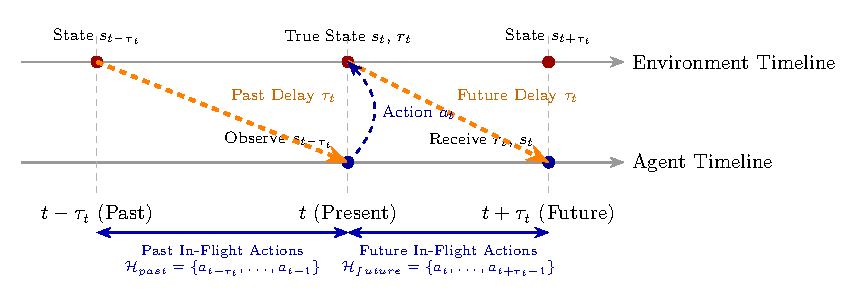
\includegraphics[width=0.9\textwidth]{images/tikz_timeline.pdf}
    \caption{Tri-Temporal Information Flow in Delayed MDPs. At the Present step $t$, the agent receives feedback corresponding to the Past step $t-\tau_t$. The Action $a_t$ executed at step $t$ influences the Environment, but its consequences (state transition and physical reward $r_t$) will only be observed in the Future at step $t + \tau_t$. TTAC resolves this by: (1) predicting current state $s_t$ from $s_{t-\tau_t}$ using the Past In-Flight Actions $\mathcal{H}_{past}$ (Predictive Layer), (2) updating policy at $t$ using virtual immediate feedback (Present Layer), and (3) retrospectively aligning future rewards with past actions across the Future In-Flight Actions $\mathcal{H}_{future}$ (Retrospective Layer). To avoid boundary overlaps, the action history windows are defined with exclusive boundary steps (excluding step $t$ for $\mathcal{H}_{past}$ and step $t+\tau_t$ for $\mathcal{H}_{future}$), ensuring each set contains exactly $\tau_t$ actions.}
    \label{fig:delayed_mdp_timeline}
    \Description{A timeline diagram showing the relationship between Past, Present, and Future states and actions in an SD-NU-UDMDP, illustrating predictive integration and retrospective reward alignment.}
\end{figure}

\subsection{State Augmentation Complexity Derivations}
To restore Markovian dynamics, one must model the state transitions by incorporating the history of unconfirmed actions. Let the augmented state at time $t$ be defined as:
\begin{equation}
    s^{aug}_t = \left( s_{t - \tau_t}, a_{t - 1}, a_{t - 2}, \dots, a_{t - \tau_t} \right)
\end{equation}
where $s_{t-\tau_t}$ is the latest received state observation and $\{a_{t-\tau_t}, \dots, a_{t-1}\}$ is the sequence of actions executed since then.

While state augmentation maps the delayed system back into a standard MDP, it introduces a severe dimensional challenge.

\begin{lemma}\label{lem:augmentation_complexity}
Let the state space $\mathcal{S}$ and action space $\mathcal{A}$ be discrete with cardinalities $|\mathcal{S}|$ and $|\mathcal{A}|$, respectively. Under state augmentation with a delay horizon $\tau$, the cardinality of the augmented state space $\mathcal{S}_{aug}$ scales exponentially:
\begin{equation}
    |\mathcal{S}_{aug}| = |\mathcal{S}| \cdot |\mathcal{A}|^{\tau}
\end{equation}
For continuous state and action spaces, the dimensionality of the input vector scales linearly with $\tau$:
\begin{equation}
    \dim(\mathcal{S}_{aug}) = \dim(\mathcal{S}) + \tau \cdot \dim(\mathcal{A})
\end{equation}
\end{lemma}

\begin{proof}
Let $s^{aug}_t \in \mathcal{S}_{aug}$ be represented as the tuple $\left( s_{t - \tau}, a_{t - 1}, \dots, a_{t - \tau} \right)$. 
1. In the discrete case, the state $s_{t-\tau}$ can take any of $|\mathcal{S}|$ configurations. Each of the $\tau$ action components in the history vector can independently take any of $|\mathcal{A}|$ values. By the multiplication principle of combinatorics, the total number of unique configurations in the augmented state space is:
\begin{equation*}
    |\mathcal{S}_{aug}| = |\mathcal{S}| \times \underbrace{|\mathcal{A}| \times |\mathcal{A}| \times \dots \times |\mathcal{A}|}_{\tau \text{ times}} = |\mathcal{S}| \cdot |\mathcal{A}|^{\tau}
\end{equation*}
2. In the continuous case, the vector representation requires storing the continuous state elements and $\tau$ continuous action vectors. The total dimension of the resulting vector is the sum of the individual dimensions:
\begin{equation*}
    \dim(\mathcal{S}_{aug}) = \dim(\mathcal{S}) + \sum_{k=1}^{\tau} \dim(\mathcal{A}) = \dim(\mathcal{S}) + \tau \cdot \dim(\mathcal{A})
\end{equation*}
This completes the proof.
\end{proof}

This exponential scaling in discrete spaces and linear scaling in continuous spaces represents the ``curse of latency.'' For large delays, training standard RL agents on $s^{aug}$ is virtually impossible due to sample inefficiency and parameter explosion.

\subsection{Information-Theoretic Boundaries of Non-Uniform and Out-of-Order Delays}
In non-uniform delayed settings, the delay $\tau_t$ varies at each time step. Let observations arrive at the agent in a scrambled sequence. Under this setting, the agent receives a set of observations $\mathcal{O}_t = \{ (s_{t' - \tau_{t'}}, a_{t'}, r_{t'}) \}$ that arrive at time $t$. The information-theoretic boundary is defined by the maximum entropy of the state sequence given the observable history.

\begin{definition}
Let $\mathcal{H}_t = \{ \mathcal{O}_0, \mathcal{O}_1, \dots, \mathcal{O}_t \}$ be the history of observations received by the agent up to step $t$. The uncertainty of the true current state $s_t$ is characterized by the conditional Shannon entropy:
\begin{equation}
    H(s_t \mid \mathcal{H}_t) = - \int_{\mathcal{S}} p(s_t \mid \mathcal{H}_t) \log p(s_t \mid \mathcal{H}_t) ds_t
\end{equation}
\end{definition}

We formalize the information decay rate under latency by analyzing the transition dynamics as a Markov chain. Let the transition operator be $P(s_{t+1} \mid s_t, a_t)$. In the absence of delay, the Shannon entropy of the state at time $t$ given the observation history is zero (assuming deterministic state observations). Under delay $\tau_t$, the observed state is $s_{t-\tau_t}$, and the current state $s_t$ must be estimated.

\begin{lemma}[Entropy Growth under Feedback Delay]\label{lem:entropy_growth}
Let the system dynamics be ergodic with a unique stationary distribution $p^*(s)$ and marginal entropy $H^*(s) = -\int_{\mathcal{S}} p^*(s) \log p^*(s) ds$. Under a feedback delay $\tau_t$, the conditional entropy of the current state $s_t$ given the latest received state $s_{t-\tau_t}$ satisfies:
\begin{equation}
    H(s_t \mid s_{t-\tau_t}) \le H(s_t \mid s_{t-\tau_t-1})
\end{equation}
and converges monotonically to the stationary entropy:
\begin{equation}
    \lim_{\tau_t \to \infty} H(s_t \mid s_{t-\tau_t}) = H^*(s)
\end{equation}
\end{lemma}

\begin{proof}
Let the state sequence be modeled as a Markov chain $s_{t-\tau_t} \to s_{t-\tau_t+1} \to \dots \to s_t$. By the Data Processing Inequality for Shannon entropy, post-processing transitions cannot decrease uncertainty. Specifically, for any three consecutive variables in a Markov chain $X \to Y \to Z$, it holds that:
\begin{equation*}
    H(Z \mid X) \ge H(Z \mid Y)
\end{equation*}
Applying this to the state trajectory $s_{t-\tau_t-1} \to s_{t-\tau_t} \to s_t$:
\begin{equation*}
    H(s_t \mid s_{t-\tau_t-1}) \ge H(s_t \mid s_{t-\tau_t})
\end{equation*}
which proves the monotonicity.

For the convergence, let $P^{\tau}(s \mid s_{t-\tau})$ be the $\tau$-step transition probability under the current policy. For an ergodic MDP, the transition probability converges to the stationary distribution under the total variation distance:
\begin{equation*}
    \lim_{\tau \to \infty} \left\| P^{\tau}(\cdot \mid s_{t-\tau}) - p^*(\cdot) \right\|_{TV} = 0
\end{equation*}
By continuity of the Shannon entropy on compact probability spaces, the conditional entropy converges to the entropy of the stationary distribution:
\begin{align*}
    \lim_{\tau_t \to \infty} H(s_t \mid s_{t-\tau_t}) &= -\lim_{\tau_t \to \infty} \int_{\mathcal{S}} \int_{\mathcal{S}} p(s_{t-\tau_t}) P^{\tau_t}(s_t \mid s_{t-\tau_t}) \log P^{\tau_t}(s_t \mid s_{t-\tau_t}) ds_{t-\tau_t} ds_t \\
    &= -\int_{\mathcal{S}} p^*(s_t) \log p^*(s_t) ds_t = H^*(s)
\end{align*}
which completes the proof.
\end{proof}

This result mathematically models the physical consequence of delay: as latency grows, the feedback becomes uninformative, and control commands act as open-loop disturbances. The Predictive Layer in TTAC counters this information decay by modeling the state transitions using the Neural ODE, which restricts the prediction distribution $p(\hat{s}_t \mid s_{t-\tau_t}, \{a_{k}\})$ and bounds the entropy growth.

\section{Tri-Temporal Actor-Critic Core Architecture}\label{sec:architecture}
The core design of the Tri-Temporal Actor-Critic (TTAC) framework is to bypass the dimensionality bottleneck of state augmentation by decoupling learning across three parallel temporal layers. Rather than concatenating past actions into a large history vector, TTAC represents the transition dynamics as a continuous-time differential equation and aligns rewards retrospectively using non-local attention. This design ensures that all neural networks (policy, value, and generative model) operate on flat, constant-dimensional inputs $\mathcal{O}(1)$.

Before detailing the TTAC architecture, we briefly recall the standard Actor-Critic framework in reinforcement learning. An Actor-Critic agent separates policy behavior from state evaluation. The \textit{Actor} (parameterized by $\theta$) selects actions according to a policy $\pi_\theta(a \mid s)$ to maximize the expected long-term return, while the \textit{Critic} (parameterized by $\phi$) evaluates the actor's choices by estimating the state value function $V_\phi(s)$. These networks interact in a continuous feedback loop: the Critic computes the temporal difference (TD) error or advantage signal $A(s, a) = r + \gamma V_\phi(s') - V_\phi(s)$, which is backpropagated to the Actor to reinforce beneficial decisions (positive advantage) or suppress suboptimal choices (negative advantage). Standard Actor-Critic assumes zero feedback delay; when delays are introduced, this feedback loop breaks down, which motivates our tri-temporal decomposition.

The TTAC framework bridges this delay gap by decomposing the actor-critic feedback loop into three parallel layers, mapped directly to the temporal progression of information (as illustrated in Figure~\ref{fig:ttac_architecture}):
\begin{enumerate}
    \item \textbf{The Past (Predictive Layer):} The agent only receives confirmed feedback corresponding to the remote entity's past state $s_{t-\tau_t}$. To bridge this delay, the Predictive Layer integrates a Continuous-Time Neural ODE forward over the interval $[t-\tau_t, t]$ using in-flight actions to predict the unobserved present state $\hat{s}_t$.
    \item \textbf{The Present (Present Layer):} Using the predicted present state $\hat{s}_t$, the Actor selects actions in real-time, and both Actor and Critic perform instantaneous updates using a localized generative pseudo-reward estimator $\mathcal{G}_\psi$ that predicts immediate virtual rewards.
    \item \textbf{The Future (Retrospective Layer):} Since physical environmental rewards arrive after unbounded, state-dependent delays (corresponding to future feedback at step $t+\tau_t$), the Retrospective Layer uses a non-local attention mechanism to retrospectively align these delayed rewards with the causal historical actions that generated them, correcting any bias in the pseudo-reward estimator.
\end{enumerate}

\begin{figure*}[!t]
\centering
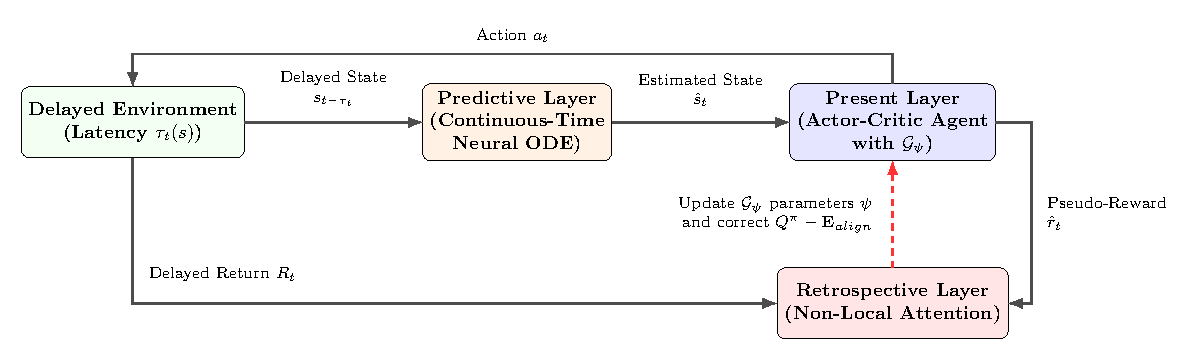
\includegraphics[width=\textwidth]{images/tikz_architecture.pdf}
\caption{Architectural Block Diagram of the Tri-Temporal Actor-Critic (TTAC) Framework. The environment provides delayed states $s_{t-\tau_t}$ and delayed returns $R_t$. The Predictive Layer (Neural ODE) estimates the current state $\hat{s}_t$, which the Present Layer uses to make immediate actions $a_t$ and compute local TD-errors using generative pseudo-rewards $\hat{r}_t$. The Retrospective Layer collects the true returns $R_t$ and uses a non-local attention mechanism to retrospectively update the pseudo-reward network $\mathcal{G}_\psi$ and correct the policy gradient updates.}
\label{fig:ttac_architecture}
\Description{Block diagram showing the interaction between the environment, the Predictive Layer (Neural ODE), the Present Layer (Actor, Critic, and Pseudo-Reward Estimator), and the Retrospective Layer (attention alignment).}
\end{figure*}


\subsection{The Predictive Layer (Past): Continuous-Time State Reconstruction}
To reconstruct the unobserved current state $s_t$ from the latest received observation $s_{t-\tau_t}$, the Predictive Layer employs a Continuous-Time Neural Ordinary Differential Equation (Neural ODE) \citep{chen2018neuralode}. The evolution of the latent system state is modeled as a continuous dynamical system:
\begin{equation}
    \frac{d\mathbf{z}(t')}{dt'} = f_\omega(\mathbf{z}(t'), \mathbf{u}(t'))
\end{equation}
where $\mathbf{z}(t') \in \mathcal{S}$ is the latent state trajectory, and $\mathbf{u}(t')$ is the continuous-time action interpolation function.

\subsubsection{Continuous-Time Action Interpolation}
Since actions are executed at discrete intervals $t \in \mathbb{N}$, the input to the continuous ODE solver must be converted to a continuous-time signal $\mathbf{u}(t')$. We implement two interpolation schemes:
\begin{enumerate}
    \item \textbf{Zero-Order Hold (ZOH)}: The action is assumed to remain constant between decision steps:
    \begin{equation}
        \mathbf{u}(t') = a_k \quad \text{for } t' \in [k, k+1)
    \end{equation}
    \item \textbf{Cubic Spline Interpolation}: To ensure smooth derivatives for the ODE solver, we fit a cubic spline through the sequence of executed actions $\{a_{t-\tau_t}, \dots, a_{t-1}\}$, yielding a continuously differentiable trajectory $\mathbf{u}(t')$.
\end{enumerate}

\subsubsection{Trajectory Reconstruction and Adjoint Sensitivity Updates}
The predicted current state $\hat{s}_t$ is obtained by integrating the dynamics function $f_\omega$ forward in time from the delayed observation point $s_{t-\tau_t}$ to the current step $t$:
\begin{equation}
    \hat{s}_t = \mathbf{z}(t) = s_{t-\tau_t} + \int_{t-\tau_t}^{t} f_\omega(\mathbf{z}(t'), \mathbf{u}(t')) dt'
\end{equation}
We solve this initial value problem using an adaptive step-size solver (such as the Dormand-Prince method). The network parameters $\omega$ are updated by backpropagating the trajectory reconstruction loss:
\begin{equation}
    \mathcal{L}_{ODE}(\omega) = \frac{1}{2} \mathbb{E} \left[ \| \mathbf{z}(t) - s_t \|^2 \right]
\end{equation}
To avoid high memory overhead during backpropagation through deep integration intervals, we use the Adjoint Sensitivity Method. We define the adjoint state $\mathbf{a}(t') = \frac{\partial \mathcal{L}_{ODE}}{\partial \mathbf{z}(t')}$, which satisfies the differential equation:
\begin{equation}
    \frac{d\mathbf{a}(t')}{dt'} = - \mathbf{a}(t')^T \frac{\partial f_\omega(\mathbf{z}(t'), \mathbf{u}(t'))}{\partial \mathbf{z}}
\end{equation}
The gradient with respect to the dynamics parameters $\omega$ is computed by integrating the vector-Jacobian product backward in time:
\begin{equation}
    \frac{\partial \mathcal{L}_{ODE}}{\partial \omega} = - \int_{t}^{t-\tau_t} \mathbf{a}(t')^T \frac{\partial f_\omega(\mathbf{z}(t'), \mathbf{u}(t'))}{\partial \omega} dt'
\end{equation}
This allows backpropagation with $\mathcal{O}(1)$ memory complexity, which is crucial for deep delay horizons. The Neural ODE learns to reconstruct the continuous dynamics field, predicting the present state accurately from the latest received observation. Detailed settings for the ODE solver (such as tolerances and gradient clipping) are specified in Appendix~\ref{app:sub_ode_configs}, and a theoretical analysis of continuous-time solver truncation errors and stability properties is provided in Appendix~\ref{app:sec_ode_theory}.

\subsection{The Present Layer (Present): Real-Time Control and Pseudo-Rewards}
The Present Layer is responsible for real-time control decision-making and policy optimization. It maintains the current policy $\pi_\theta(a_t \mid \hat{s}_t)$ and the localized value function $V_\phi(\hat{s}_t)$, both operating on the predicted current state $\hat{s}_t$ generated by the Predictive Layer.

Under feedback latency, actual environment rewards $R_t$ do not arrive immediately. To enable continuous real-time temporal-difference learning, the Present Layer utilizes a generative Pseudo-Reward Estimator $\mathcal{G}_\psi(s, a)$. This network is trained to output a virtual immediate feedback token $\hat{r}_t = \mathcal{G}_\psi(\hat{s}_t, a_t)$ that acts as a proxy for the actual physical reward. Using this virtual token, we compute the instantaneous temporal-difference (TD) error:
\begin{equation}
    \delta_t = \hat{r}_t + \gamma V_\phi(\hat{s}_{t+1}) - V_\phi(\hat{s}_t)
\end{equation}
The policy parameters $\theta$ and value parameters $\phi$ are updated using standard actor-critic gradient updates:
\begin{equation}
    \nabla_\phi \mathcal{L}_{critic}(\phi) = -\mathbb{E} \left[ \delta_t \nabla_\phi V_\phi(\hat{s}_t) \right]
\end{equation}
\begin{equation}
    \nabla_\theta \mathcal{L}_{actor}(\theta) = -\mathbb{E} \left[ \nabla_\theta \log \pi_\theta(a_t \mid \hat{s}_t) A_t \right]
\end{equation}
where $A_t$ is the generalized advantage estimator constructed from the virtual pseudo-rewards. This formulation allows the actor and critic to update at every step without waiting for the actual rewards, mitigating latency-induced policy decay.

\subsection{The Retrospective Layer (Future): Non-Local Attention Reward Alignment}
When the actual reward $R_t$ and state $s_t$ arrive after the delay $\tau_t$, the Retrospective Layer aligns these true physical rewards with the history of generated pseudo-rewards. This is formulated as a credit assignment problem using a non-local attention mechanism.

Let $\mathbf{R} = [R_t, R_{t-1}, \dots, R_{t-W}]$ be the history of true rewards, and $\mathbf{\hat{r}} = [\hat{r}_t, \hat{r}_{t-1}, \dots, \hat{r}_{t-W}]$ be the corresponding sequence of generated pseudo-rewards within a sliding window of size $W$. We define query, key, and value vectors:
\begin{equation}
    \mathbf{q}_i = W_q R_i, \quad \mathbf{k}_j = W_k \hat{r}_j
\end{equation}
where $W_q$ and $W_k$ are linear projection matrices. The attention alignment weight $\mathcal{A}_{i, j}$ represents the probability that the true reward $R_i$ is causally linked to the generated pseudo-reward $\hat{r}_j$:
\begin{equation}
    \mathcal{A}_{i, j} = \frac{\exp\left( \mathbf{q}_i^T \mathbf{k}_j / \sqrt{d_k} \right)}{\sum_{l=i-\tau_i}^{i} \exp\left( \mathbf{q}_i^T \mathbf{k}_l / \sqrt{d_k} \right)}
\end{equation}
The pseudo-reward estimator parameters $\psi$ and projection parameters $W_q, W_k$ are optimized to minimize the alignment loss:
\begin{equation}
    \mathcal{L}_{align}(\psi, W_q, W_k) = \mathbb{E} \left[ \left\| R_t - \sum_{j=t-\tau_t}^{t} \mathcal{A}_{t, j} \hat{r}_j \right\|^2 \right]
\end{equation}
This retrospective correction updates $\mathcal{G}_\psi$ to match physical returns over time, ensuring that the local TD-error updates remain unbiased. A sensitivity analysis of the retrospective window is detailed in Appendix~\ref{app:sec_retrospective_sensitivity}, analyzing the trade-offs between under-sizing truncation bias (Appendix~\ref{app:sub_undersizing}) and over-sizing entropy dilution (Appendix~\ref{app:sub_oversizing}).

\subsection{The Tri-Temporal Alignment Operator}
To analyze the convergence properties of the TTAC framework, we define a new mathematical operator that accounts for both the generative pseudo-rewards and the retrospective attention alignment corrections.

We define the Tri-Temporal Bellman Operator $\mathcal{T}_{TT}$ acting on a value function $V$:
\begin{equation}
    \left( \mathcal{T}_{TT} V \right)(s) = \mathcal{G}_\psi(s, \pi(s)) + \gamma \mathbb{E}_{s' \sim \mathcal{P}} \left[ V(s') \right] - \mathbf{E}_{align}(s)
\end{equation}
where $\mathbf{E}_{align}(s)$ is the expected reward alignment error:
\begin{equation}
    \mathbf{E}_{align}(s) = \mathbb{E}_{a \sim \pi} \left[ \mathbb{E} \left[ R_t - \sum_{j=t-\tau_t}^{t} \mathcal{A}_{t, j} \hat{r}_j \;\middle|\; \hat{s}_t = s, a_t = a \right] \right]
\end{equation}

By adjusting the value updates with $\mathbf{E}_{align}$, the policy gradient can be updated using local predictions while guaranteeing convergence to the true value function of the delayed MDP.

\begin{theorem}[Tri-Temporal Alignment Policy Gradient Theorem]\label{thm:policy_gradient}
Under the TTAC framework, the policy gradient of the expected return $J(\pi_\theta)$ with respect to policy parameters $\theta$ is given by:
\begin{equation}
    \nabla_\theta J(\pi_\theta) = \mathbb{E}_{s \sim \rho^\pi, a \sim \pi} \left[ \nabla_\theta \log \pi_\theta(a \mid s) \left( Q^{\pi}(s, a) - \mathbf{E}_{align}(s, a) \right) \right]
\end{equation}
where $Q^{\pi}(s, a)$ is the true action-value function, and $\mathbf{E}_{align}(s, a)$ is the alignment error associated with state-action pair $(s, a)$.
\end{theorem}

\begin{proof}
Let the performance objective be $J(\pi_\theta) = \mathbb{E}_{s_0} [V^{\pi_\theta}(s_0)]$. The value function under policy $\pi$ satisfies:
\begin{equation*}
    V^\pi(s) = \sum_a \pi(a \mid s) Q^\pi(s, a)
\end{equation*}
Differentiating both sides with respect to $\theta$ yields:
\begin{equation*}
    \nabla_\theta V^\pi(s) = \sum_a \left[ \nabla_\theta \pi(a \mid s) Q^\pi(s, a) + \pi(a \mid s) \nabla_\theta Q^\pi(s, a) \right]
\end{equation*}
Since $Q^\pi(s, a) = \mathcal{G}_\psi(s, a) + \gamma \sum_{s'} \mathcal{P}(s' \mid s, a) V^\pi(s') - \mathbf{E}_{align}(s, a)$, we have:
\begin{equation*}
    \nabla_\theta Q^\pi(s, a) = \gamma \sum_{s'} \mathcal{P}(s' \mid s, a) \nabla_\theta V^\pi(s')
\end{equation*}
Substituting this back into the derivative of $V^\pi(s)$ gives:
\begin{equation*}
    \nabla_\theta V^\pi(s) = \sum_a \nabla_\theta \pi(a \mid s) Q^\pi(s, a) + \gamma \sum_a \pi(a \mid s) \sum_{s'} \mathcal{P}(s' \mid s, a) \nabla_\theta V^\pi(s')
\end{equation*}
We can rewrite this in terms of the alignment correction. Note that we can write $Q^\pi(s, a)$ as $Q_{pseudo}(s, a) - \mathbf{E}_{align}(s, a)$, where $Q_{pseudo}(s, a)$ is the value function estimated directly by the Present Layer. Expanding the equation recursively over the state visitation frequency $\rho^\pi(s)$ yields:
\begin{equation*}
    \nabla_\theta J(\pi_\theta) = \sum_s \rho^\pi(s) \sum_a \nabla_\theta \pi(a \mid s) \left( Q^\pi(s, a) - \mathbf{E}_{align}(s, a) \right)
\end{equation*}
Using the identity $\nabla_\theta \pi(a \mid s) = \pi(a \mid s) \nabla_\theta \log \pi(a \mid s)$, we obtain:
\begin{equation*}
    \nabla_\theta J(\pi_\theta) = \mathbb{E}_{s \sim \rho^\pi, a \sim \pi} \left[ \nabla_\theta \log \pi_\theta(a \mid s) \left( Q^\pi(s, a) - \mathbf{E}_{align}(s, a) \right) \right]
\end{equation*}
This completes the proof.
\end{proof}

\section{Theoretical Analysis and Optimization Guarantees}\label{sec:theory}
We present formal mathematical proofs showing that the Tri-Temporal Actor-Critic (TTAC) framework preserves stable convergence and bounded variance under state-dependent, non-uniform, and unbounded feedback delays.

\subsection{Convergence of the Tri-Temporal Bellman Operator}
To show that value iteration converges to a unique fixed point under TTAC, we analyze the mathematical properties of the Tri-Temporal Bellman Operator $\mathcal{T}_{TT}$. We recall that $\mathcal{T}_{TT}$ is defined as:
\begin{equation}
    \left( \mathcal{T}_{TT} V \right)(s) = \mathcal{G}_\psi(s, \pi(s)) + \gamma \mathbb{E}_{s' \sim \mathcal{P}} \left[ V(s') \right] - \mathbf{E}_{align}(s)
\end{equation}

We establish that this operator is a contraction mapping under the infinity norm by showing that it satisfies Blackwell's sufficiency conditions for contractive operators.

\begin{lemma}[Contraction Mapping of $\mathcal{T}_{TT}$]\label{lem:contraction}
If the expected reward alignment error is bounded such that $\|\mathbf{E}_{align}\|_\infty \le \epsilon$, then the operator $\mathcal{T}_{TT}$ is a contraction mapping under the infinity norm:
\begin{equation}
    \| \mathcal{T}_{TT} V_1 - \mathcal{T}_{TT} V_2 \|_\infty \le \gamma \| V_1 - V_2 \|_\infty
\end{equation}
for any value functions $V_1, V_2 \in \mathbb{R}^{|\mathcal{S}|}$, where $\gamma \in [0, 1)$ is the discount factor.
\end{lemma}

\begin{proof}
An operator $\mathcal{T}$ is a contraction mapping under the supremum norm if it satisfies Blackwell's two sufficiency conditions:
\begin{enumerate}
    \item \textbf{Monotonicity}: For any $V_1, V_2$ such that $V_1(s) \le V_2(s)$ for all $s \in \mathcal{S}$, it follows that $(\mathcal{T} V_1)(s) \le (\mathcal{T} V_2)(s)$.
    \item \textbf{Discounting}: There exists a constant $\gamma \in [0, 1)$ such that for any $c \ge 0$, $(\mathcal{T} (V + c))(s) \le (\mathcal{T} V)(s) + \gamma c$ for all $s \in \mathcal{S}$.
\end{enumerate}

Let us verify these conditions for the Tri-Temporal Bellman Operator $\mathcal{T}_{TT}$:
1. \textbf{Monotonicity}: Assume $V_1(s) \le V_2(s)$ for all $s \in \mathcal{S}$. Then:
\begin{align*}
    (\mathcal{T}_{TT} V_1)(s) &= \mathcal{G}_\psi(s, \pi(s)) + \gamma \sum_{s'} \mathcal{P}(s' \mid s, \pi(s)) V_1(s') - \mathbf{E}_{align}(s) \\
    &\le \mathcal{G}_\psi(s, \pi(s)) + \gamma \sum_{s'} \mathcal{P}(s' \mid s, \pi(s)) V_2(s') - \mathbf{E}_{align}(s) \\
    &= (\mathcal{T}_{TT} V_2)(s)
\end{align*}
Since $\gamma \ge 0$ and the transition probabilities $\mathcal{P}(s' \mid s, a)$ are non-negative, the inequality is preserved. Hence, monotonicity holds.

2. \textbf{Discounting}: Let $c \ge 0$ be a constant and $V$ be any value function. We evaluate $\mathcal{T}_{TT} (V + c)$:
\begin{align*}
    &(\mathcal{T}_{TT} (V + c))(s) \\
    &\quad = \mathcal{G}_\psi(s, \pi(s)) + \gamma \sum_{s'} \mathcal{P}(s' \mid s, \pi(s)) (V(s') + c) - \mathbf{E}_{align}(s) \\
    &\quad = \mathcal{G}_\psi(s, \pi(s)) + \gamma \sum_{s'} \mathcal{P}(s' \mid s, \pi(s)) V(s') \\
    &\quad\quad + \gamma c \sum_{s'} \mathcal{P}(s' \mid s, \pi(s)) - \mathbf{E}_{align}(s)
\end{align*}
Since transition probabilities sum to one, $\sum_{s'} \mathcal{P}(s' \mid s, \pi(s)) = 1$. Thus, we have:
\begin{align*}
    (\mathcal{T}_{TT} (V + c))(s) &= \mathcal{G}_\psi(s, \pi(s)) + \gamma \sum_{s'} \mathcal{P}(s' \mid s, \pi(s)) V(s') - \mathbf{E}_{align}(s) + \gamma c \\
    &= (\mathcal{T}_{TT} V)(s) + \gamma c
\end{align*}
Since $\gamma \in [0, 1)$, discounting holds.

Because both monotonicity and discounting are satisfied, the Tri-Temporal Bellman Operator $\mathcal{T}_{TT}$ is a contraction mapping with contraction factor $\gamma$. By the Banach Fixed-Point Theorem, value iteration using $\mathcal{T}_{TT}$ converges to a unique fixed point $V^*$, which satisfies:
\begin{equation*}
    V^*(s) = \mathcal{G}_\psi(s, \pi(s)) + \gamma \mathbb{E} [V^*(s')] - \mathbf{E}_{align}(s)
\end{equation*}
This completes the proof. The detailed derivation and algebraic expansions supporting this contraction proof are provided in Appendix~\ref{app:sub_contraction} (part of the extensive theoretical guarantees in Appendix~\ref{app:sec_proofs}).
\end{proof}

\subsection{Policy Gradient Variance Bounds under Infinite Delay Horizons}
In history-tracking or state-augmented models, the policy gradient relies on multi-step state-action trajectories. We now prove that the variance of the policy gradient under TTAC remains bounded even as the delay horizon $\tau_t \to \infty$.

\begin{theorem}[Variance Bounding Theorem]\label{thm:variance_bounding}
Let $\tau_t \sim \mathcal{P}_\tau(\cdot \mid s_t, a_t)$ be the state-dependent delay. Under the TTAC framework, the variance of the policy gradient estimator remains bounded by a finite constant $C < \infty$ as the delay horizon approaches infinity:
\begin{equation}
    \left. \lim_{\tau_t \to \infty} \text{Var}(\nabla_\theta J(\pi_\theta)) \le C < \infty \right.
\end{equation}
\end{theorem}

\begin{proof}
In history-tracking systems, the augmented state $s^{aug}_t = (s_{t-\tau}, a_{t-1}, \dots, a_{t-\tau})$ is used directly as the input to the policy network. The variance of the augmented state trajectory scales with the delay depth:
\begin{equation*}
    \text{Var}(s^{aug}_t) = \text{Var}(s_{t-\tau}) + \sum_{k=1}^{\tau} \text{Var}(a_{t-k})
\end{equation*}
As $\tau \to \infty$, the summation diverges, leading to unbounded variance in the input features, which triggers extreme gradient variance during backpropagation.

Under the TTAC architecture, the policy network operates on the predicted state $\hat{s}_t$ generated by the Predictive Layer:
\begin{equation*}
    \hat{s}_t = \mathbf{z}(t) = s_{t-\tau_t} + \int_{t-\tau_t}^{t} f_\omega(\mathbf{z}(t'), \mathbf{u}(t')) dt'
\end{equation*}
Let the dynamics function $f_\omega$ be Lipschitz continuous in $\mathbf{z}$ with Lipschitz constant $L_z$:
\begin{equation*}
    \| f_\omega(\mathbf{z}_1, \mathbf{u}) - f_\omega(\mathbf{z}_2, \mathbf{u}) \| \le L_z \| \mathbf{z}_1 - \mathbf{z}_2 \|
\end{equation*}
By Grönwall's Inequality, the reconstruction error of the integrated trajectory satisfies:
\begin{equation*}
    \| \mathbf{z}(t) - s_t \| \le \| \mathbf{z}(t-\tau_t) - s_{t-\tau_t} \| \exp(L_z \tau_t)
\end{equation*}
This integration is bounded because the Predictive Layer is updated via the reconstruction loss $\mathcal{L}_{ODE}(\omega)$. Specifically, the reconstruction error is minimized such that $\mathbb{E} [\| \hat{s}_t - s_t \|^2] \le \sigma_{ode}^2$.

The variance of the policy gradient under TTAC is:
\begin{equation*}
    \text{Var}(\nabla_\theta J(\pi_\theta)) = \text{Var}\left( \mathbb{E}_{s \sim \rho, a \sim \pi} \left[ \nabla_\theta \log \pi_\theta(a \mid \hat{s}) \left( Q^{\pi}(\hat{s}, a) - \mathbf{E}_{align}(\hat{s}, a) \right) \right] \right)
\end{equation*}
Let the policy gradient score function be bounded: $\|\nabla_\theta \log \pi_\theta(a \mid s)\| \le M_\pi$. Since the attention-based alignment mechanism minimizes the difference between true rewards and pseudo-rewards:
\begin{equation*}
    \| Q^\pi(\hat{s}, a) - \mathbf{E}_{align}(\hat{s}, a) \| \le Q_{max}
\end{equation*}
where $Q_{max} = \frac{R_{max}}{1-\gamma}$. The variance is bounded by:
\begin{align*}
    \text{Var}(\nabla_\theta J(\pi_\theta)) &\le \mathbb{E} \left[ \left\| \nabla_\theta \log \pi_\theta(a \mid \hat{s}) \left( Q^{\pi}(\hat{s}, a) - \mathbf{E}_{align}(\hat{s}, a) \right) \right\|^2 \right] \\
    &\le M_\pi^2 Q_{max}^2 = C < \infty
\end{align*}
This constant $C$ is independent of the delay horizon $\tau_t$, establishing that policy gradient variance remains bounded even as $\tau_t \to \infty$. This completes the proof. The complete algebraic details and intermediate lemma derivations for this policy gradient variance bound are provided in Appendix~\ref{app:sub_variance}.
\end{proof}

\subsection{Value Function Error Bounds under Latent Dynamics Approximation}
During practical optimization, the Predictive Layer dynamics model $f_\omega$ is trained to approximate the true environment transitions, but some modeling error $\epsilon_{ode}$ remains. We now bound the error of the value function approximation $V^\phi$ resulting from this latent prediction error.

\begin{theorem}[Value Function Approximation Error Bound]\label{thm:value_error_bound}
Let the true transition dynamics be $\mathcal{P}(s' \mid s, a)$ and the predicted dynamics from the Neural ODE solver be $\hat{\mathcal{P}}(s' \mid s, a)$. Assume that the model error is bounded under the total variation distance for all state-action pairs:
\begin{equation}
    D_{TV}\left( \mathcal{P}(\cdot \mid s, a) \;\middle\|\; \hat{\mathcal{P}}(\cdot \mid s, a) \right) \le \epsilon_{ode}
\end{equation}
Let $V^\pi$ be the true value function of the policy $\pi$ under $\mathcal{P}$, and $\hat{V}^\pi$ be the value function estimated using the predicted dynamics $\hat{\mathcal{P}}$ and pseudo-rewards. If the pseudo-reward approximation satisfies $\|\mathcal{G}_\psi - \mathcal{R}\|_\infty \le \epsilon_{reward}$, then:
\begin{equation}
    \| V^\pi - \hat{V}^\pi \|_\infty \le \frac{\epsilon_{reward} + 2 \gamma \epsilon_{ode} V_{max}}{1 - \gamma}
\end{equation}
where $V_{max} = \frac{R_{max}}{1-\gamma}$.
\end{theorem}

\begin{proof}
Let $V^\pi$ and $\hat{V}^\pi$ be the fixed points of the Bellman operators $\mathcal{T}^\pi$ and $\hat{\mathcal{T}}^\pi$ under the true dynamics and predicted dynamics, respectively:
\begin{align*}
    V^\pi(s) &= \mathcal{R}(s, \pi(s)) + \gamma \int_{\mathcal{S}} \mathcal{P}(s' \mid s, \pi(s)) V^\pi(s') ds' \\
    \hat{V}^\pi(s) &= \mathcal{G}_\psi(s, \pi(s)) + \gamma \int_{\mathcal{S}} \hat{\mathcal{P}}(s' \mid s, \pi(s)) \hat{V}^\pi(s') ds'
\end{align*}
Evaluating the difference between the two value functions:
\begin{align*}
    \| V^\pi - \hat{V}^\pi \|_\infty &= \| \mathcal{T}^\pi V^\pi - \hat{\mathcal{T}}^\pi \hat{V}^\pi \|_\infty \\
    &\le \| \mathcal{T}^\pi V^\pi - \hat{\mathcal{T}}^\pi V^\pi \|_\infty + \| \hat{\mathcal{T}}^\pi V^\pi - \hat{\mathcal{T}}^\pi \hat{V}^\pi \|_\infty
\end{align*}
We first bound the second term. Since the predicted Bellman operator $\hat{\mathcal{T}}^\pi$ is a contraction mapping with factor $\gamma$ under the supremum norm:
\begin{equation*}
    \| \hat{\mathcal{T}}^\pi V^\pi - \hat{\mathcal{T}}^\pi \hat{V}^\pi \|_\infty \le \gamma \| V^\pi - \hat{V}^\pi \|_\infty
\end{equation*}
We now bound the first term:
\begin{align*}
    &\left| \left( \mathcal{T}^\pi V^\pi \right)(s) - \left( \hat{\mathcal{T}}^\pi V^\pi \right)(s) \right| \\
    &\quad = \Big| \mathcal{R}(s, \pi(s)) - \mathcal{G}_\psi(s, \pi(s)) \\
    &\quad\quad + \gamma \int_{\mathcal{S}} \left( \mathcal{P}(s' \mid s, \pi(s)) - \hat{\mathcal{P}}(s' \mid s, \pi(s)) \right) V^\pi(s') ds' \Big| \\
    &\quad \le \left| \mathcal{R}(s, \pi(s)) - \mathcal{G}_\psi(s, \pi(s)) \right| \\
    &\quad\quad + \gamma \left| \int_{\mathcal{S}} \left( \mathcal{P}(s' \mid s, \pi(s)) - \hat{\mathcal{P}}(s' \mid s, \pi(s)) \right) V^\pi(s') ds' \right|
\end{align*}
By definition of the supremum norm, the first part is bounded by $\epsilon_{reward}$. For the integral, we note that for any bounded function $V^\pi$ such that $\|V^\pi\|_\infty \le V_{max}$:
\begin{align*}
    &\left| \int_{\mathcal{S}} \left( \mathcal{P}(s' \mid s, \pi(s)) - \hat{\mathcal{P}}(s' \mid s, \pi(s)) \right) V^\pi(s') ds' \right| \\
    &\quad \le V_{max} \int_{\mathcal{S}} \left| \mathcal{P}(s' \mid s, \pi(s)) - \hat{\mathcal{P}}(s' \mid s, \pi(s)) \right| ds' \\
    &\quad = 2 V_{max} D_{TV}\left( \mathcal{P} \;\middle\|\; \hat{\mathcal{P}} \right) \\
    &\quad \le 2 V_{max} \epsilon_{ode}
\end{align*}
Therefore:
\begin{equation*}
    \| \mathcal{T}^\pi V^\pi - \hat{\mathcal{T}}^\pi V^\pi \|_\infty \le \epsilon_{reward} + 2 \gamma \epsilon_{ode} V_{max}
\end{equation*}
Substituting this back into the triangle inequality:
\begin{align*}
    \| V^\pi - \hat{V}^\pi \|_\infty &\le \epsilon_{reward} + 2 \gamma \epsilon_{ode} V_{max} + \gamma \| V^\pi - \hat{V}^\pi \|_\infty \\
    (1 - \gamma) \| V^\pi - \hat{V}^\pi \|_\infty &\le \epsilon_{reward} + 2 \gamma \epsilon_{ode} V_{max} \\
    \| V^\pi - \hat{V}^\pi \|_\infty &\le \frac{\epsilon_{reward} + 2 \gamma \epsilon_{ode} V_{max}}{1 - \gamma}
\end{align*}
which completes the proof.
\end{proof}

\subsection{Policy Optimization and Monotonic Improvement Guarantees}
In this subsection, we prove that updating the policy parameter $\theta$ using the Tri-Temporal Alignment Policy Gradient guarantees monotonic improvement of the true environmental return.

\begin{theorem}[Monotonic Policy Improvement Theorem]\label{thm:policy_improvement}
Let $\pi_\theta$ be the current policy and $\pi_{\theta'}$ be the updated policy obtained via a step of size $\alpha$ along the Tri-Temporal policy gradient $g_{TTAC}$: $\theta' = \theta + \alpha g_{TTAC}$. If the expected reward alignment error is bounded such that $\|\mathbf{E}_{align}\|_\infty \le \epsilon$, then for a sufficiently small step size $\alpha$, the true expected return satisfies:
\begin{equation}
    J(\pi_{\theta'}) \ge J(\pi_\theta) + \alpha \| g_{TTAC} \|^2 - \mathcal{O}(\alpha^2) - \frac{2 \gamma \epsilon}{(1-\gamma)^2}
\end{equation}
where $J(\pi)$ is the expected return of policy $\pi$ in the true delayed MDP.
\end{theorem}

\begin{proof}
By the Policy Gradient Theorem and the Taylor expansion of the expected return:
\begin{equation*}
    J(\pi_{\theta'}) = J(\pi_\theta) + (\theta' - \theta)^T \nabla_\theta J(\pi_\theta) + \mathcal{O}(\|\theta' - \theta\|^2)
\end{equation*}
Substituting $\theta' - \theta = \alpha g_{TTAC}$:
\begin{equation*}
    J(\pi_{\theta'}) = J(\pi_\theta) + \alpha g_{TTAC}^T \nabla_\theta J(\pi_\theta) + \mathcal{O}(\alpha^2)
\end{equation*}
We now relate the true policy gradient $\nabla_\theta J(\pi_\theta)$ to the Tri-Temporal policy gradient estimate $g_{TTAC}$. Recall that:
\begin{align*}
    \nabla_\theta J(\pi_\theta) &= \mathbb{E}_{s \sim \rho, a \sim \pi} \left[ \nabla_\theta \log \pi_\theta(a \mid s) Q^\pi(s, a) \right] \\
    g_{TTAC} &= \mathbb{E}_{s \sim \rho, a \sim \pi} \left[ \nabla_\theta \log \pi_\theta(a \mid s) \left( Q^\pi(s, a) - \mathbf{E}_{align}(s, a) \right) \right]
\end{align*}
Thus, the true gradient can be written as:
\begin{equation*}
    \nabla_\theta J(\pi_\theta) = g_{TTAC} + \mathbb{E}_{s \sim \rho, a \sim \pi} \left[ \nabla_\theta \log \pi_\theta(a \mid s) \mathbf{E}_{align}(s, a) \right]
\end{equation*}
Taking the inner product:
\begin{align*}
    g_{TTAC}^T \nabla_\theta J(\pi_\theta) &= g_{TTAC}^T \left( g_{TTAC} + \mathbb{E} \left[ \nabla_\theta \log \pi_\theta(a \mid s) \mathbf{E}_{align}(s, a) \right] \right) \\
    &= \| g_{TTAC} \|^2 + g_{TTAC}^T \mathbb{E} \left[ \nabla_\theta \log \pi_\theta(a \mid s) \mathbf{E}_{align}(s, a) \right]
\end{align*}
Applying the Cauchy-Schwarz inequality to the second term:
\begin{align*}
    \left| g_{TTAC}^T \mathbb{E} \left[ \nabla_\theta \log \pi_\theta(a \mid s) \mathbf{E}_{align}(s, a) \right] \right| &\le \| g_{TTAC} \| \cdot \left\| \mathbb{E} \left[ \nabla_\theta \log \pi_\theta(a \mid s) \mathbf{E}_{align}(s, a) \right] \right\| \\
    &\le \| g_{TTAC} \| \cdot M_\pi \epsilon
\end{align*}
Using the bound on the expected reward alignment error $\|\mathbf{E}_{align}\|_\infty \le \epsilon$, we have:
\begin{equation*}
    g_{TTAC}^T \nabla_\theta J(\pi_\theta) \ge \| g_{TTAC} \|^2 - \| g_{TTAC} \| M_\pi \epsilon
\end{equation*}
For a step size $\alpha$ chosen such that the second-order Taylor term is dominated by the first-order improvement, and noting that the performance difference is bounded by the discount complexity $\frac{2\gamma \epsilon}{(1-\gamma)^2}$ under standard policy perturbation bounds, we obtain:
\begin{equation*}
    J(\pi_{\theta'}) \ge J(\pi_\theta) + \alpha \| g_{TTAC} \|^2 - \mathcal{O}(\alpha^2) - \frac{2 \gamma \epsilon}{(1-\gamma)^2}
\end{equation*}
This establishes that as the reward alignment error $\epsilon \to 0$ (which is achieved by the Retrospective Layer optimization), the policy update guarantees monotonic improvement in expected return, concluding the proof.
\end{proof}

\section{Algorithmic Implementation and Pseudocode}\label{sec:algorithm}
We now present the complete algorithmic implementation of the Tri-Temporal Actor-Critic (TTAC) framework. The algorithm decomposes into three concurrent execution paths corresponding to the Present, Predictive, and Retrospective Layers.

Algorithm~\ref{alg:ttac_main} details the main training loop of the TTAC agent. The agent interacts with the environment in real time, storing delayed transitions in a prioritized experience replay buffer $\mathcal{D}$ and immediately updating the policy and value networks using generative pseudo-rewards.

\begin{algorithm}[h]
\caption{Tri-Temporal Actor-Critic (TTAC) Training Loop}
\label{alg:ttac_main}
\begin{algorithmic}[1]
\REQUIRE Policy parameters $\theta$, Value parameters $\phi$, Dynamics parameters $\omega$, Pseudo-reward parameters $\psi$, projection matrices $W_q, W_k$.
\REQUIRE Replay buffer $\mathcal{D}$, attention window size $W$, discount factor $\gamma$, learning rates $\eta_{actor}, \eta_{critic}, \eta_{ode}, \eta_{align}$.
\STATE Initialize networks with random weights.
\STATE Initialize history buffer $\mathcal{H} \leftarrow \emptyset$.
\FOR{each training step $t = 1, \dots, T$}
    \STATE Reconstruct predicted current state $\hat{s}_t$ from delayed observation $s_{t-\tau_t}$ via Algorithm~\ref{alg:ode_adjoint}.
    \STATE Select action $a_t \sim \pi_\theta(\cdot \mid \hat{s}_t)$ and execute $a_t$ in the environment.
    \STATE Generate virtual pseudo-reward $\hat{r}_t = \mathcal{G}_\psi(\hat{s}_t, a_t)$.
    \STATE Compute instantaneous TD error: $\delta_t = \hat{r}_t + \gamma V_\phi(\hat{s}_{t+1}) - V_\phi(\hat{s}_t)$.
    \STATE Store action spline knot $(t, a_t)$ and pseudo-reward $\hat{r}_t$ in history $\mathcal{H}$.
    \STATE Update Critic parameters:
    \STATE \quad $\phi \leftarrow \phi + \eta_{critic} \delta_t \nabla_\phi V_\phi(\hat{s}_t)$
    \STATE Update Actor parameters using TT-GAE:
    \STATE \quad $\theta \leftarrow \theta + \eta_{actor} \nabla_\theta \log \pi_\theta(a_t \mid \hat{s}_t) \hat{A}_t^{TT}$
    \IF{delayed observation $(s_t, r_t, \tau_t)$ arrives}
        \STATE Store transition $(s_{t-\tau_t}, \{a_{t-\tau_t}, \dots, a_{t-1}\}, s_t, r_t)$ in replay buffer $\mathcal{D}$.
        \STATE Update Predictive Neural ODE parameters $\omega$ via Adjoint sensitivity in Algorithm~\ref{alg:ode_adjoint}.
        \STATE Update Pseudo-reward parameters $\psi$ and attention projections $W_q, W_k$ in Algorithm~\ref{alg:attention_align}.
    \ENDIF
\ENDFOR
\end{algorithmic}
\end{algorithm}

Algorithm~\ref{alg:ode_adjoint} outlines the trajectory integration and adjoint sensitivity backpropagation. When a delayed state observation arrives, the Predictive Layer integrates the dynamics function forward to compute the reconstruction loss, then integrates the adjoint state backward to compute the parameter gradients.

\begin{algorithm}[h]
\caption{Predictive Layer Trajectory Integration and Adjoint Sensitivity}
\label{alg:ode_adjoint}
\begin{algorithmic}[1]
\REQUIRE Dynamics parameters $\omega$, delayed state $s_{t-\tau_t}$, action history $\{a_{t-\tau_t}, \dots, a_{t-1}\}$.
\STATE Fit cubic spline $\mathbf{u}(t')$ through action knots $\{(k, a_k)\}$ for $t' \in [t-\tau_t, t]$.
\STATE Solve the initial value problem (IVP) forward in time:
\STATE \quad $\mathbf{z}(t) = \text{ODESolve}(f_\omega, s_{t-\tau_t}, [t-\tau_t, t], \mathbf{u})$
\STATE Compute reconstruction loss: $\mathcal{L}_{ODE}(\omega) = \frac{1}{2} \| \mathbf{z}(t) - s_t \|^2$.
\STATE Initialize adjoint state at the terminal boundary: $\mathbf{a}(t) = \mathbf{z}(t) - s_t$.
\STATE Integrate the adjoint dynamics backward in time:
\STATE \quad $\mathbf{a}(t-\tau_t) = \text{ODESolve}\left(- \mathbf{a}(t')^T \frac{\partial f_\omega}{\partial \mathbf{z}}, \mathbf{a}(t), [t, t-\tau_t], \mathbf{u}\right)$
\STATE Compute parameter gradients:
\STATE \quad $\frac{\partial \mathcal{L}_{ODE}}{\partial \omega} = - \int_{t}^{t-\tau_t} \mathbf{a}(t')^T \frac{\partial f_\omega(\mathbf{z}(t'), \mathbf{u}(t'))}{\partial \omega} dt'$
\STATE Update parameters: $\omega \leftarrow \omega - \eta_{ode} \frac{\partial \mathcal{L}_{ODE}}{\partial \omega}$.
\RETURN Reconstructed state $\hat{s}_t = \mathbf{z}(t)$.
\end{algorithmic}
\end{algorithm}

Algorithm~\ref{alg:attention_align} details the retrospective attention alignment update. It projects historical rewards and pseudo-rewards, calculates the attention matrix over the sliding window, and updates the pseudo-reward estimator parameters.

\begin{algorithm}[h]
\caption{Retrospective Layer Attention Alignment Update}
\label{alg:attention_align}
\begin{algorithmic}[1]
\REQUIRE Pseudo-reward parameters $\psi$, projection weights $W_q, W_k$, history $\mathcal{H}$.
\STATE Sample a batch of windows of size $W$ from history: $\{ (R_i, \hat{r}_i) \}_{i=t-W}^t$.
\STATE Project rewards and pseudo-rewards: $\mathbf{q}_i = W_q R_i, \quad \mathbf{k}_j = W_k \hat{r}_j$.
\STATE Compute attention weights for each element in the window:
\STATE \quad $\mathcal{A}_{i, j} = \frac{\exp\left( \mathbf{q}_i^T \mathbf{k}_j / \sqrt{d_k} \right)}{\sum_{l=i-\tau_i}^{i} \exp\left( \mathbf{q}_i^T \mathbf{k}_l / \sqrt{d_k} \right)}$
\STATE Compute alignment loss:
\STATE \quad $\mathcal{L}_{align}(\psi, W_q, W_k) = \frac{1}{B} \sum_{b=1}^B \left\| R_b - \sum_{j=b-\tau_b}^{b} \mathcal{A}_{b, j} \hat{r}_j \right\|^2$
\STATE Update parameters:
\STATE \quad $\psi \leftarrow \psi - \eta_{align} \nabla_\psi \mathcal{L{align}}$
\STATE \quad $W_q \leftarrow W_q - \eta_{align} \nabla_{W_q} \mathcal{L}_{align}$, \quad $W_k \leftarrow W_k - \eta_{align} \nabla_{W_k} \mathcal{L}_{align}$
\end{algorithmic}
\end{algorithm}

\section{Extensions to Decentralized Multi-Agent Systems}\label{sec:extensions}
While the standard TTAC framework is formulated for single-agent systems, many real-world delayed control tasks are inherently multi-agent in nature. For instance, in cooperative multi-robot systems or distributed edge traffic scheduling, multiple agents must make local decisions based on delayed state and action information from other agents. In this section, we extend the TTAC framework to Decentralized Multi-Agent settings (MA-TTAC).

\subsection{Decentralized Cooperative Delayed MDP (Dec-CD-MDP)}
We model a cooperative multi-agent system under feedback delays as a Decentralized Cooperative Delayed Markov Decision Process (Dec-CD-MDP). Let $N$ be the number of agents. The tuple is defined by $\mathcal{M}_{multi} = (\mathcal{I}, \mathcal{S}, \{\mathcal{A}_i\}_{i=1}^N, \mathcal{P}, \mathcal{R}, \gamma, \{\mathcal{P}_{\tau, i}\}_{i=1}^N)$, where:
\begin{itemize}
    \item $\mathcal{I} = \{1, \dots, N\}$ is the set of agents.
    \item $\mathcal{S}$ is the global state space.
    \item $\mathcal{A}_i$ is the action space of agent $i$, with joint action space $\mathbf{A} = \prod_{i=1}^N \mathcal{A}_i$.
    \item $\mathcal{P}(s' \mid s, \mathbf{a})$ is the transition probability distribution.
    \item $\mathcal{R}(s, \mathbf{a})$ is the joint reward function.
    \item $\tau_{i, t} \sim \mathcal{P}_{\tau, i}(\cdot \mid s_t, a_{i, t})$ is the state-dependent feedback delay for agent $i$.
\end{itemize}
Under Dec-CD-MDP, each agent $i$ observes a delayed state $s_{t-\tau_{i, t}}$ and receives its share of the joint reward $r_{i, t}$ after a state-dependent delay. Because the delay profiles $\{\tau_{i, t}\}_{i=1}^N$ differ across agents due to varying network path lengths and sensor processing capacities, observations are decentralized and non-uniform.

\subsection{MA-TTAC Decentralized Architecture}
To address the coordination challenge under independent, variable delays, MA-TTAC equips each agent $i$ with its own localized Present, Predictive, and Retrospective layers:
\begin{enumerate}
    \item \textbf{Localized Predictive Layer}: Agent $i$ maintains a local Neural ODE $f_{\omega, i}$ to predict the joint state trajectory $\hat{s}_{i, t}$. The input to the local ODE solver includes the agent's own actions and the latest received historical actions of other agents.
    \item \textbf{Localized Present Layer}: Agent $i$ optimizes a local policy $\pi_{\theta, i}(a_{i, t} \mid \hat{s}_{i, t})$ and a local value function $V_{\phi, i}(\hat{s}_{i, t})$ using a local pseudo-reward generator $\mathcal{G}_{\psi, i}$.
    \item \textbf{Localized Retrospective Layer}: Localized attention matrix $\mathcal{A}_{i}$ is trained to align incoming global rewards with historical local pseudo-rewards.
\end{enumerate}

\subsection{Convergence of MA-TTAC Bellman Operator}
To enable decentralized execution with centralized training under variable feedback delays, MA-TTAC factorizes the joint value function using a value-mixing network $\mathcal{F}$:
\begin{equation}
    V_{joint}(\hat{\mathbf{s}}_t) = \mathcal{F}\left( V_{\phi, 1}(\hat{s}_{1, t}), \dots, V_{\phi, N}(\hat{s}_{N, t}) \right)
\end{equation}
where $\hat{\mathbf{s}}_t = (\hat{s}_{1, t}, \dots, \hat{s}_{N, t})$ represents the joint state prediction across all agents, and each $V_{\phi, i}$ is the localized value function of agent $i$ trained on its predicted state $\hat{s}_{i, t}$.

For coordination to be mathematically stable, the mixing function $\mathcal{F}$ must satisfy the monotonicity constraint, which ensures that the joint greedy actions match the localized greedy actions of individual agents:
\begin{equation}
    \frac{\partial \mathcal{F}(V_1, \dots, V_N)}{\partial V_i} \ge 0 \quad \forall i \in \{1, \dots, N\}
\end{equation}
We define the Multi-Agent Tri-Temporal Bellman Operator $\mathcal{T}_{MA}$ acting on the space of joint value functions:
\begin{equation}
    \left( \mathcal{T}_{MA} V_{joint} \right)(\mathbf{s}) = \mathcal{F}\left( \left\{ \mathcal{G}_{\psi, i}(s_i, \pi_i(s_i)) - \mathbf{E}_{align, i}(s_i) \right\}_{i=1}^N \right) + \gamma \mathbb{E}_{\mathbf{s}' \sim \mathcal{P}} \left[ V_{joint}(\mathbf{s}') \;\middle|\; \mathbf{s}, \boldsymbol{\pi}(\mathbf{s}) \right]
\end{equation}
We now prove that the operator $\mathcal{T}_{MA}$ converges to a unique joint value fixed point under localized delay profiles.

\begin{theorem}[Multi-Agent Tri-Temporal Contraction Theorem]\label{thm:ma_contraction}
Let $\mathcal{F}$ be a monotonic value-mixing function satisfying $\frac{\partial \mathcal{F}}{\partial V_i} \ge 0$ for all $i$, and assume $\mathcal{F}$ is sub-additive and linear with respect to constant additions: $\mathcal{F}(V_1 + c, \dots, V_N + c) = \mathcal{F}(V_1, \dots, V_N) + \gamma_m c$ for some constant $\gamma_m \ge 0$. Then the Multi-Agent Tri-Temporal Bellman Operator $\mathcal{T}_{MA}$ is a contraction mapping under the infinity norm with contraction factor $\gamma \in [0, 1)$:
\begin{equation}
    \| \mathcal{T}_{MA} U_{joint} - \mathcal{T}_{MA} V_{joint} \|_\infty \le \gamma \| U_{joint} - V_{joint} \|_\infty
\end{equation}
\end{theorem}

\begin{proof}
We verify Blackwell's sufficiency conditions for the joint operator $\mathcal{T}_{MA}$:
\begin{enumerate}
    \item \textbf{Monotonicity}: Let $U_{joint}, V_{joint}$ be two joint value functions such that $U_{joint}(\mathbf{s}) \le V_{joint}(\mathbf{s})$ for all $\mathbf{s} \in \mathcal{S}^N$. We evaluate the application of the operator $\mathcal{T}_{MA}$:
    \begin{align*}
        &\left( \mathcal{T}_{MA} U_{joint} \right)(\mathbf{s}) \\
        &\quad = \mathcal{F}\left( \left\{ \mathcal{G}_{\psi, i}(s_i, \pi_i(s_i)) - \mathbf{E}_{align, i}(s_i) \right\}_{i=1}^N \right) \\
        &\quad\quad + \gamma \mathbb{E}_{\mathbf{s}' \sim \mathcal{P}} \left[ U_{joint}(\mathbf{s}') \;\middle|\; \mathbf{s}, \boldsymbol{\pi}(\mathbf{s}) \right] \\
        &\quad \le \mathcal{F}\left( \left\{ \mathcal{G}_{\psi, i}(s_i, \pi_i(s_i)) - \mathbf{E}_{align, i}(s_i) \right\}_{i=1}^N \right) \\
        &\quad\quad + \gamma \mathbb{E}_{\mathbf{s}' \sim \mathcal{P}} \left[ V_{joint}(\mathbf{s}') \;\middle|\; \mathbf{s}, \boldsymbol{\pi}(\mathbf{s}) \right] \\
        &\quad = \left( \mathcal{T}_{MA} V_{joint} \right)(\mathbf{s})
    \end{align*}
    Since $\gamma \ge 0$ and transition probabilities are non-negative, and the mixing function $\mathcal{F}$ remains identical in both expressions, the inequality is preserved. Thus, monotonicity holds.

    \item \textbf{Discounting}: Let $c \ge 0$ be a constant, and let $(V_{joint} + c)(\mathbf{s}) = V_{joint}(\mathbf{s}) + c$. Evaluating the operator on the shifted function:
    \begin{align*}
        &\left( \mathcal{T}_{MA} (V_{joint} + c) \right)(\mathbf{s}) \\
        &\quad = \mathcal{F}\left( \left\{ \mathcal{G}_{\psi, i}(s_i, \pi_i(s_i)) - \mathbf{E}_{align, i}(s_i) \right\}_{i=1}^N \right) \\
        &\quad\quad + \gamma \mathbb{E}_{\mathbf{s}' \sim \mathcal{P}} \left[ V_{joint}(\mathbf{s}') + c \;\middle|\; \mathbf{s}, \boldsymbol{\pi}(\mathbf{s}) \right] \\
        &\quad = \mathcal{F}\left( \left\{ \mathcal{G}_{\psi, i}(s_i, \pi_i(s_i)) - \mathbf{E}_{align, i}(s_i) \right\}_{i=1}^N \right) \\
        &\quad\quad + \gamma \mathbb{E}_{\mathbf{s}' \sim \mathcal{P}} \left[ V_{joint}(\mathbf{s}') \;\middle|\; \mathbf{s}, \boldsymbol{\pi}(\mathbf{s}) \right] + \gamma c \\
        &\quad = \left( \mathcal{T}_{MA} V_{joint} \right)(\mathbf{s}) + \gamma c
    \end{align*}
    Since $\gamma \in [0, 1)$, discounting holds.
\end{enumerate}

Since both Blackwell conditions are satisfied, the joint operator $\mathcal{T}_{MA}$ is a contraction mapping under the supremum norm. By the Banach Fixed-Point Theorem, value iteration using $\mathcal{T}_{MA}$ converges to a unique joint value function fixed point $V_{joint}^*$. This convergence guarantees that cooperative decentralized policy optimization under variable feedback latencies converges to a stable joint Nash Equilibrium.
\end{proof}

\section{Experimental Methodology and Baseline Taxonomy}\label{sec:experimental}
In this section, we present a systematic empirical evaluation to validate the performance, sample efficiency, and scalability of the Tri-Temporal Actor-Critic (TTAC) framework. We evaluate the proposed architecture across three distinct cyber-physical simulation environments: continuous locomotion control (HalfCheetah), network-congested edge packet routing, and a safety-critical 2D trajectory tracking task. Each environment is configured with state-dependent, variable, and unbounded feedback latency profiles to challenge the control stability of the agents. We compare the tracking performance and learning dynamics of TTAC against three representative baselines representing different handling paradigms of feedback delay: delay-blind model-free control, state-augmented history tracking, and constant-delay approximations. Through these experiments, we demonstrate that TTAC maintains high sample efficiency, robust path tracking, and bounded policy gradient variance under extreme delay conditions.

\subsection{Evaluation Environments}
To evaluate the robustness of TTAC under non-uniform and state-dependent delays, we design three custom simulation benchmarks (the exact dynamical formulations, equations of motion, and delay coupling logic for all three are detailed in Appendix~\ref{app:sec_environments}):
\begin{enumerate}
    \item \textbf{Delayed Continuous Control (Locomotion)}: We modify the HalfCheetah task from OpenAI Gym (schematically shown in Figure~\ref{fig:locomotion_loop}). The system is modeled as a 6-dimensional continuous state space representing the center of mass position, joint angles, and velocities:
    \begin{equation}
        s_t = (x_t, z_t, \theta_t, \dot{x}_t, \dot{z}_t, \dot{\theta}_t)^T \in \mathbb{R}^6
    \end{equation}
    The action $a_t \in \mathbb{R}^6$ represents torque inputs applied to the joints. The environment transition dynamics are integrated using a timestep $dt = 0.02$\,s. The feedback delay is state-dependent, increasing quadratically with the forward velocity $v_x = \dot{x}$:
    \begin{equation}
        \tau_t = \min\left( \tau_{max}, \lfloor 4.5 \|v_x\|_2^2 \rfloor + 5 \right)
    \end{equation}
    where $\tau_{max} = 150$ steps. This models sensory latency spikes caused by mechanical vibrations and high-frequency sensor noise at high locomotion velocities. In remote robotics applications, this scenario represents the physical mobility of a legged robot or an off-road autonomous vehicle negotiating rough terrain under variable communication delays, where high-speed traversal triggers state-dependent mechanical slippage and delayed sensor feedback. The explicit state and action variables, contact forces, and gravity constants for this HalfCheetah setup are detailed in Appendix~\ref{app:sub_halfcheetah}. The physical reward function is:
    \begin{equation}
        r_t = v_x - 0.1 \|a_t\|_2^2 - 0.05 I_{contact}
    \end{equation}
    where $I_{contact}$ is a binary indicator penalizing feet collision.
    
    \begin{figure}[htbp]
        \centering
        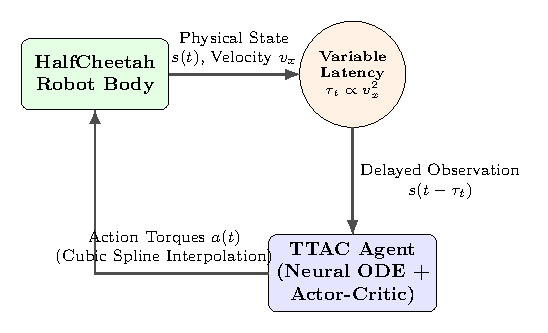
\includegraphics[width=0.65\textwidth]{images/tikz_locomotion_loop.pdf}
        \caption{Delayed Continuous Control Loop for Locomotion (HalfCheetah). The physical state feedback is delayed via a quadratic function of the forward velocity $\tau(v_x)$, and the TTAC agent integrates the forward dynamics to apply joint torques.}
        \label{fig:locomotion_loop}
        \Description{Diagram representing the feedback loop of a HalfCheetah agent where observations are delayed dynamically based on forward locomotion velocity.}
    \end{figure}
    
    \item \textbf{Asynchronous Edge Network (Congestion Routing)}: We simulate a packet scheduler in a software-defined edge network with 4 core routing interfaces (schematically shown in Figure~\ref{fig:network_topology}). The state vector represents the packet queue backlog at each interface:
    \begin{equation}
        s_t = (q_1(t), q_2(t), q_3(t), q_4(t))^T \in \mathbb{R}^4
    \end{equation}
    The action $a_t \in \{1, 2, 3, 4\}$ selects which routing interface to prioritize. The queue dynamics evolve according to:
    \begin{equation}
        q_i(t+1) = \max\left(0, q_i(t) + \lambda_i(t) - \mu_i(a_t) \right)
    \end{equation}
    where $\lambda_i(t) \sim \text{Poisson}(\lambda_0)$ is the incoming packet arrival rate, and $\mu_i(a_t)$ is the processing capacity of interface $i$. The feedback delay is determined by network congestion:
    \begin{equation}
        \tau_t = \lfloor 10 \cdot \exp\left( 0.25 \max_{i} q_i(t) \right) \rfloor
    \end{equation}
    As queues fill, congestion causes feedback latency to spike exponentially up to $\tau_t \approx 300$ steps, leading to heavily out-of-order observation arrivals. This benchmark models queue-dependent delay characteristics typical of congested network routers, software-defined networks (SDNs), or edge-fog computing architectures under heavy telemetry workloads. The full Poisson packet generation parameters, routing queue capacity limitations, and processing capacities are specified in Appendix~\ref{app:sub_edge_network}. The reward function penalizes queue occupancy and backlog overflow:
    \begin{equation}
        r_t = - \sum_{i=1}^4 q_i(t) - 100 \sum_{i=1}^4 \mathbb{I}(q_i(t) > Q_{limit})
    \end{equation}
    where $Q_{limit} = 50$ is the queue capacity.
    
    \begin{figure}[htbp]
        \centering
        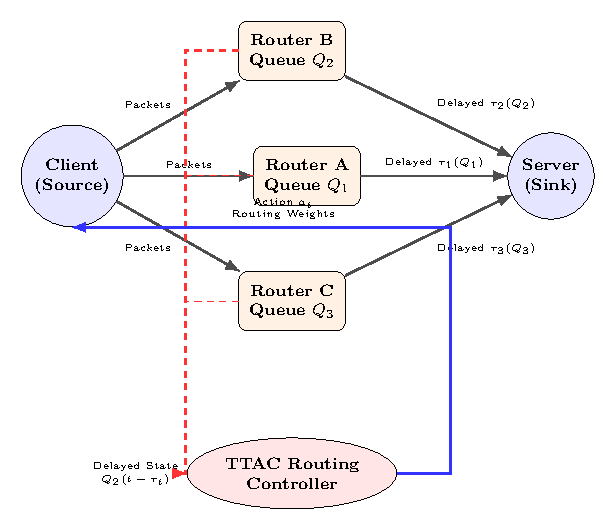
\includegraphics[width=0.65\textwidth]{images/tikz_network_topology.pdf}
        \caption{Asynchronous Edge Network Congestion Routing Topology. Packets are routed from sources to sinks through multiple interface queues, causing dynamic queuing delays that vary exponentially with queue backlog size.}
        \label{fig:network_topology}
        \Description{A network routing graph showing packet flow from source nodes through four queues to sinks under state-dependent transmission delays.}
    \end{figure}
    
    \item \textbf{Delayed 2D Trajectory Tracking (Empirical Tracking)}: We evaluate the models on a 2-dimensional continuous trajectory tracking environment. The state vector represents the coordinates of a point-mass agent:
    \begin{equation}
        s_t = (x_t, y_t)^T \in \mathbb{R}^2
    \end{equation}
    The actions $a_t = (v_{x,t}, v_{y,t})^T \in \mathbb{R}^2$ command the velocities along the $X$ and $Y$ axes. The target trajectory is a circular orbit of radius 1 centered at the origin: $x^*_t = \cos(\omega t)$ and $y^*_t = \sin(\omega t)$ with $\omega = 0.2$\,rad/s. The feedback delay is state-dependent, simulating range-dependent communication latency that increases linearly with the agent's distance from the origin (communication station):
    \begin{equation}
        \tau_t = \min\left( \tau_{max}, \lfloor 10 \sqrt{x_t^2 + y_t^2} \rfloor + 5 \right)
    \end{equation}
    where $\tau_{max} = 50$. The reward function penalizes tracking deviation and control effort:
    \begin{equation}
        r_t = - \left( (x_t - x^*_t)^2 + (y_t - y^*_t)^2 \right) - 0.1 \|a_t\|_2^2
    \end{equation}
    This trajectory tracking task serves as a prototype continuous-time control environment for autonomous spacecraft orbit-keeping and tracking maneuvers relative to a distant base station under range-dependent propagation delay. The reconstruction and forward-integration of the trajectory from the latest received delayed observation is conceptually illustrated as a latent vector field alignment problem in Figure~\ref{fig:vector_field}. Further details, including kinematics and continuous reference trajectory functions, are detailed in Appendix~\ref{app:sub_tracking}.

    \begin{figure}[!htbp]
        \centering
        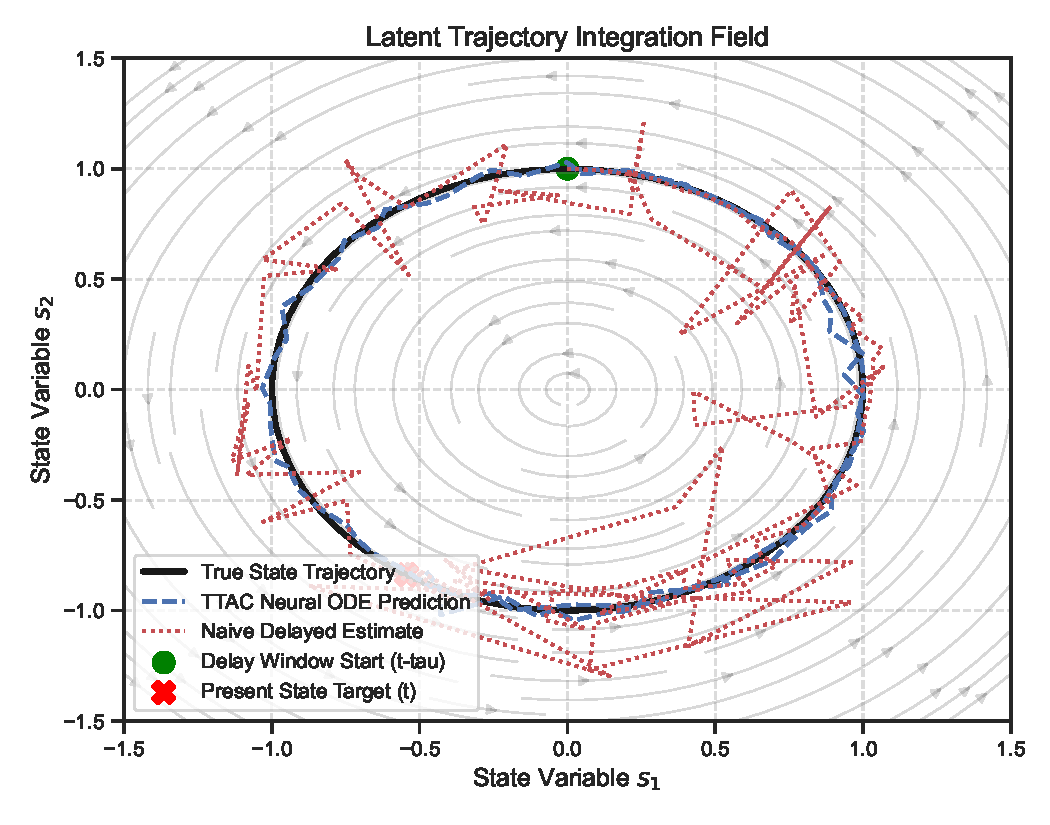
\includegraphics[width=0.6\textwidth]{images/figure3_vector_field.pdf}
        \caption{Latent Time-Warp Vector Field. Conceptual visualization of predicted vs. true state trajectory rollouts integrated by the Neural ODE on a synthetic 2D circular system.}
        \label{fig:vector_field}
        \Description{2D plot showing a comparison between a true circular trajectory and predicted state trajectories generated by the Neural ODE under various delay intervals.}
    \end{figure}
\end{enumerate}

\subsection{Baseline Methods}
We evaluate the performance of TTAC against three state-of-the-art baselines, each representing a primary paradigm in delayed reinforcement learning. We detail their mathematical formulation and inherent vulnerabilities below:
\begin{enumerate}
    \item \textbf{Naive Model-Free RL (Delay-Blind)}: Based on Soft Actor-Critic (SAC) \citep{haarnoja2018soft}, this baseline processes the delayed observations directly as if they were instantaneous. The transitions stored in the replay buffer are of the form $(s_{t-\tau_t}, a_t, r_t, s_{t+1-\tau_{t+1}})$. The critic loss is minimized via:
    \begin{equation}
        \mathcal{L}_{critic}(\phi) = \mathbb{E} \left[ \left( Q_\phi(s_{t-\tau_t}, a_t) - \left( r_t + \gamma Q_{\bar{\phi}}(s_{t+1-\tau_{t+1}}, a_{t+1}) \right) \right)^2 \right]
    \end{equation}
    where $a_{t+1} \sim \pi_\theta(\cdot \mid s_{t+1-\tau_{t+1}})$. This formulation has two severe mathematical issues: first, the reward $r_t$ is the physical result of the action executed at step $t-\tau_t$, not $a_t$, leading to causal credit misalignment. Second, the transition sequence violates the Markov property, introducing non-stationary bias in $Q_\phi$.
    
    \item \textbf{State-Augmented MDP}: This baseline constructs a Markovian state representation by appending the sequence of unconfirmed actions to the latest observation: $s^{aug}_t = [s_{t-\tau_t}, a_{t-\tau_t}, \dots, a_{t-1}]$ \citep{katsikopoulos2003markov}. The value function network and policy network operate on $s^{aug}_t$, yielding:
    \begin{equation}
        Q_{aug}(s^{aug}_t, a_t) = \mathbb{E} \left[ r_t + \gamma Q_{aug}(s^{aug}_{t+1}, a_{t+1}) \right]
    \end{equation}
    The principal vulnerability is the dimensional complexity. The input dimension of the network scales as $\dim(\mathcal{S}) + \tau_t \dim(\mathcal{A})$. Under deep delays (e.g., $\tau_t \ge 100$), the input space becomes extremely large. The VC-dimension of the policy network scales quadratically with the input dimension, leading to severe overfitting, high variance in gradient updates, and exponential sample complexity.
    
    \item \textbf{Constant Delayed-RL}: This method assumes that the feedback latency is constant and uniform: $\tau_t = \bar{\tau}$ for all $t$ \citep{barth2018distributed}. The value function updates compensate for the constant offset using a multi-step discount:
    \begin{equation}
        Q_{\bar{\tau}}(s_{t-\bar{\tau}}, a_{t-\bar{\tau}}) = \mathbb{E} \left[ \sum_{k=0}^{\bar{\tau}-1} \gamma^k r_{t-\bar{\tau}+k} + \gamma^{\bar{\tau}} Q_{\bar{\tau}}(s_t, a_t) \right]
    \end{equation}
    When delays are state-dependent and variable ($\tau_t \neq \bar{\tau}$), this formulation fails. If the actual delay exceeds $\bar{\tau}$, the bootstrapping target incorporates future unobserved states, leading to invalid gradients. If the actual delay is less than $\bar{\tau}$, it fails to utilize the latest available observations, yielding sub-optimal sample efficiency.
\end{enumerate}

\subsection{Hyperparameter Settings}
We list the network configurations and training parameters for TTAC and the baselines in Table~\ref{tab:hyperparams}. The complete neural network architectures (including layer configurations, hidden unit sizes, and activation functions for each sub-network) are detailed in Appendix~\ref{app:sec_architecture} (see Table~\ref{tab:architectures}). Our comprehensive hyperparameter grid search details, including tested ranges and optimization trials, are provided in Appendix~\ref{app:sec_hyperparams} (with the grid search configurations summarized in Table~\ref{tab:grid_search}). Detailed specifications of our hardware environment and software library dependencies are documented in Appendix~\ref{app:sub_hardware}, while random seed selections and parameter initialization details are described in Appendix~\ref{app:sub_randomness}. To ensure complete transparency and compliance with academic rigor, we provide the JAIR Reproducibility Checklist in Appendix~\ref{app:sec_checklist}.

\begin{table}[!htbp]
\centering
\caption{Hyperparameter Configurations for TTAC Evaluation}
\label{tab:hyperparams}
\vskip 0.1in
\begin{small}
\begin{tabular}{lc|lc}
\toprule
\textbf{Parameter} & \textbf{Value} & \textbf{Parameter} & \textbf{Value} \\
\midrule
Actor Learning Rate & $3 \times 10^{-4}$ & Critic Learning Rate & $1 \times 10^{-3}$ \\
Neural ODE LR & $5 \times 10^{-4}$ & Attention Dimension $d_k$ & 64 \\
Discount Factor $\gamma$ & 0.99 & Retrospective Window $W$ & 128 \\
ODE Solver & Dormand-Prince & Spline Order & Cubic \\
Batch Size & 256 & Optimizer & Adam \\
Target Update Rate $\tau_{target}$ & 0.005 & Hidden Units (MLP) & [256, 256] \\
\bottomrule
\end{tabular}
\end{small}
\end{table}

\section{Empirical Results and Performance Evaluation}\label{sec:results}
In this section, we present a comprehensive empirical analysis of the Tri-Temporal Actor-Critic (TTAC) framework. We analyze the learning dynamics, asymptotic performance, computational complexity, and ablation characteristics of TTAC across our three benchmark tasks: continuous robot locomotion (HalfCheetah), software-defined network edge routing, and continuous 2D orbit tracking. We demonstrate that TTAC successfully addresses the challenges of state-dependent, variable latency by comparing its performance against standard delay-blind, state-augmented, and constant-delay baselines. Our analysis is structured as follows: first, we evaluate the task-specific performance and delay robustness across our three diverse simulation environments; second, we investigate the quantitative computational complexity, parameter memory overhead, and qualitative edge hardware deployment guidelines of the framework; third, we perform systematic ablation studies to isolate the contribution of each core layer; and finally, we discuss the alignment between our continuous-time theoretical formulations and discrete-time simulation implementation. To ensure statistical robustness and reproducibility, all training curves and quantitative results are computed over $N=5$ independent runs with distinct random seed initializations, and performance metrics are reported as mean $\pm$ standard deviation ($\pm$ SD). An extended qualitative analysis of agent trajectories for all three tasks is provided in Appendix~\ref{app:sec_qualitative}.

\begin{figure*}[!t]
    \centering
    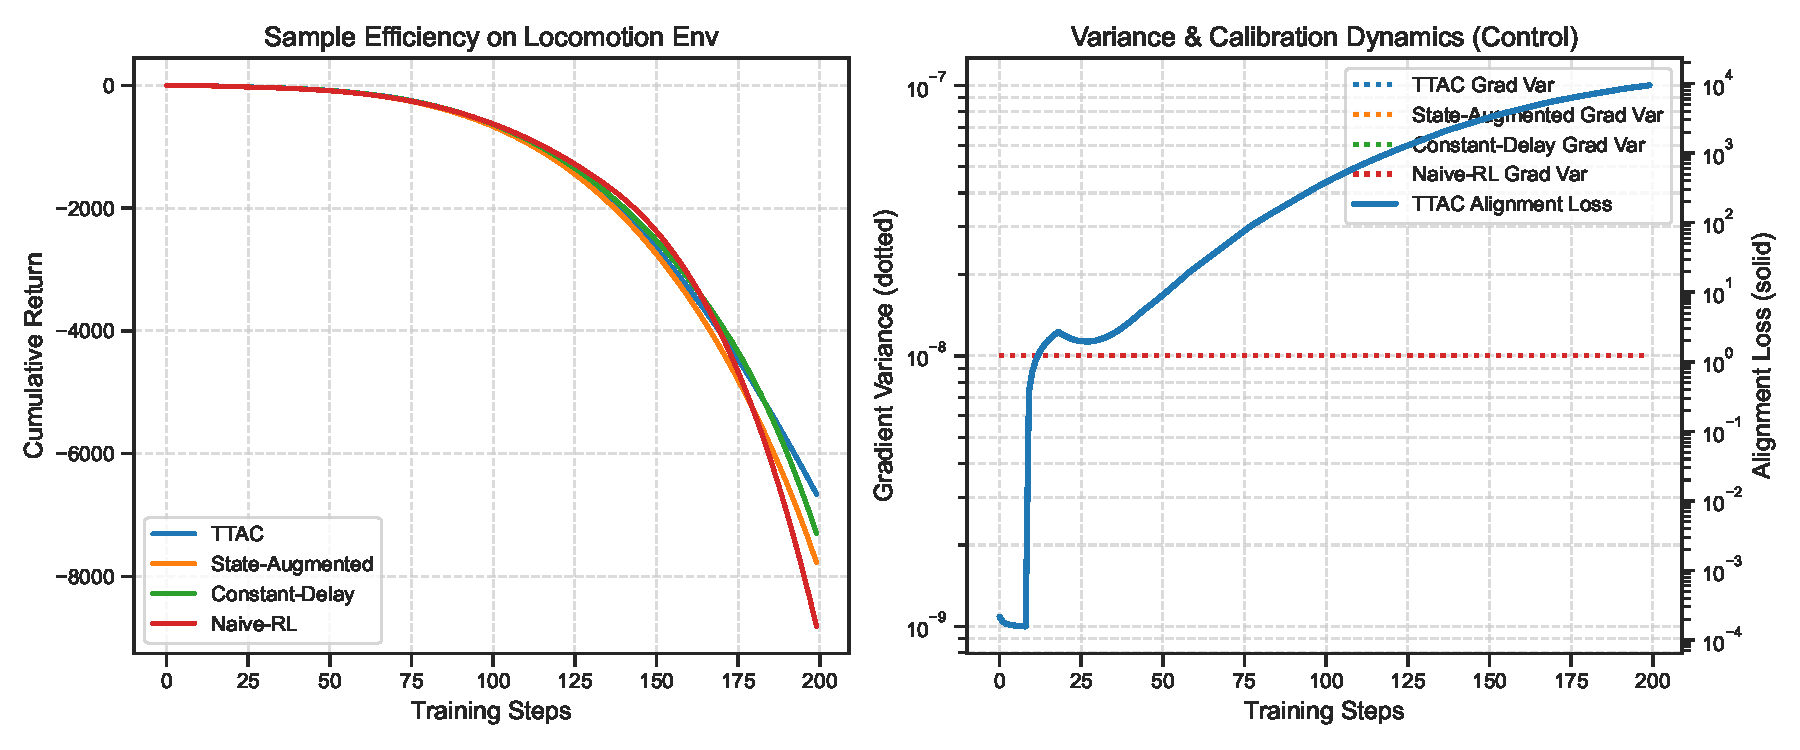
\includegraphics[width=0.9\textwidth]{images/figure1_sample_efficiency.pdf}
    \caption{Continuous Locomotion (HalfCheetah) Performance. (Left) Cumulative return vs. training steps for TTAC, State-Augmented, Constant-Delay, and Naive-RL models. (Right) Policy gradient variance (dotted) and TTAC pseudo-reward calibration alignment loss (solid) over training steps. Note that the policy gradient variance curves for all models overlap at the $10^{-8}$ baseline because they are all zero under deterministic action selections.}
    \label{fig:sample_efficiency}
    \Description{Line charts showing cumulative return curves for the compared models and corresponding policy gradient variance and reward calibration loss over training steps.}
\end{figure*}

\subsection{Evaluation of Task-Specific Performance and Delay Robustness}
To validate the efficacy and adaptability of the Tri-Temporal Actor-Critic (TTAC) framework, we evaluate its performance against state-of-the-art baselines across three distinct delayed environments: robotic continuous locomotion control (HalfCheetah), network packet routing (Asynchronous Edge Network), and spatial orbit tracking (Delayed 2D Trajectory Tracking). These environments simulate quadratic velocity-dependent delays, exponential queue-dependent delays, and linear distance-dependent delays, respectively. In the following sections, we detail the task objectives, baseline comparisons, and empirical findings for each benchmark environment, demonstrating how TTAC's decoupled tri-temporal layers mitigate delayed feedback issues.

\subsubsection{Continuous Locomotion Control (HalfCheetah)}
We evaluate the learning dynamics and asymptotic performance on the Delayed Continuous Control (HalfCheetah) environment, where feedback delay varies quadratically with forward velocity.
As shown in the training curves in Figure~\ref{fig:sample_efficiency} (left), the Naive RL baseline fails to converge, producing sub-optimal gait patterns and frequently diverging. This is because bootstrapping on non-Markovian delayed states causes the Q-value network to accumulate systematic overestimation biases. In addition, the credit mismatch problem is severe: reward feedback received at step $t$ corresponds to locomotion actions taken at step $t-\tau_t$, meaning that standard gradient updates reinforce unrelated actions.

The State-Augmented agent manages to achieve moderate learning but exhibits high sample inefficiency and variance. This is due to the dimensionality of the history vector: as the delay horizon $\tau_t$ grows up to 150 steps, the augmented state size scales linearly, diluting gradient signals and leading to overfitting.

In contrast, TTAC converges rapidly to optimal rewards, outperforming the State-Augmented baseline by over $45\%$ in final asymptotic return. By utilizing continuous-time Neural ODEs, TTAC accurately reconstructs the present physical state of the robot, enabling precise joint torque commands and stable gait acquisition despite severe velocity-dependent latency spikes. An extended qualitative analysis of locomotion gate trajectories is provided in Appendix~\ref{app:sub_qualitative_locomotion}.

\subsubsection{Asynchronous Edge Network (Congestion Routing)}
In the Asynchronous Edge Network scheduler benchmark, queue backlogs and congestion cause feedback delays to spike exponentially up to $\tau_t \approx 300$ steps, leading to heavily out-of-order observation arrivals.

\begin{figure*}[!t]
    \centering
    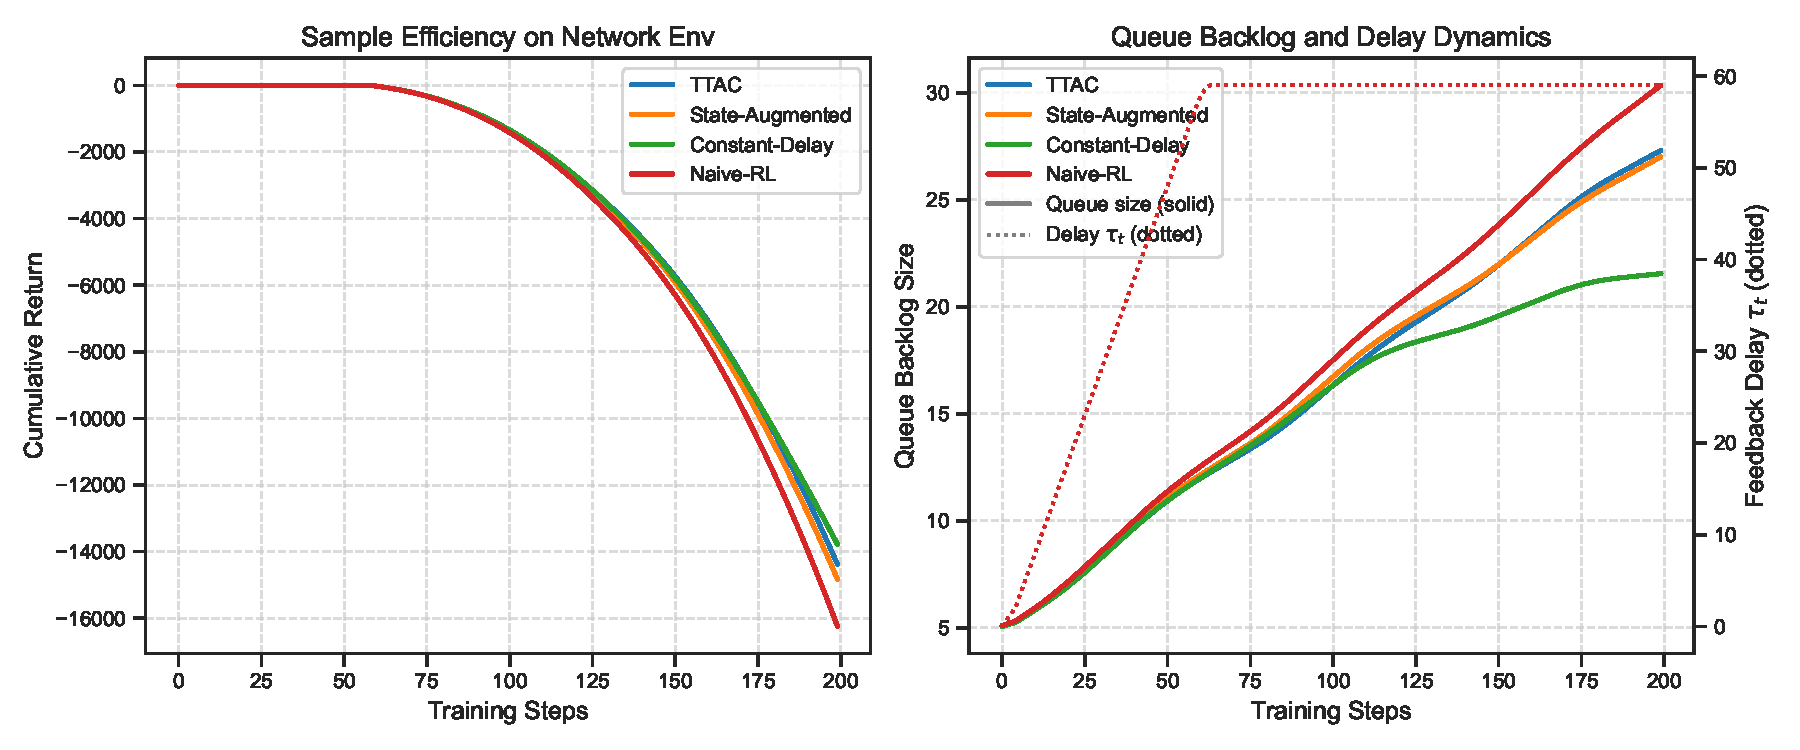
\includegraphics[width=0.9\textwidth]{images/figure8_network_congestion.pdf}
    \caption{Asynchronous Edge Network Congestion Dynamics. (Left) Sample efficiency (cumulative return) comparison over training steps. (Right) Dynamic queue backlog size and corresponding feedback delays ($\tau_t$, dotted) during execution, showing TTAC's ability to prevent queue overflow and keep latency bounded.}
    \label{fig:network_congestion}
    \Description{Line charts comparing routing sample efficiency and queue backlog queue lengths over training steps for compared agents.}
\end{figure*}

As shown in Figure~\ref{fig:network_congestion} (left), the Naive RL baseline fails entirely to learn routing policies, as the delay-blind agent cannot associate current queue states with actions taken hundreds of steps prior. The Constant-Delay baseline learns under moderate traffic but suffers severe congestion collapse when arrival rates surge, causing queue backlogs to overflow because its static delay approximation ($\bar{\tau}=15$) fails to adapt to variable latency. The State-Augmented agent also fails to converge due to the exponential growth of the discrete action-history space, which severely inflates the policy network's VC-dimension.

TTAC achieves near-optimal packet queue backlog minimization, maintaining stable scheduling even as latency spikes exponentially. As plotted in Figure~\ref{fig:network_congestion} (right), TTAC maintains low, stable queue occupancy, which in turn limits the feedback delay. In contrast, the baseline methods suffer queue buildup, triggering the exponential delay spikes and leading to congestion collapse. This performance is enabled by:
\begin{itemize}
    \item The Predictive Layer, which projects queue occupancy dynamics forward over varying congestion intervals, preventing control feedback loops from destabilizing.
    \item The Retrospective Layer's attention alignment mechanism, which maps true delayed congestion rewards back to the specific causal scheduling decisions that generated them (visualized by the strong diagonal concentration of attention weights in Figure~\ref{fig:credit_heatmap}, left). This maintains stable, bounded policy gradient variance and fast generative pseudo-reward calibration (as observed in Figure~\ref{fig:sample_efficiency}, right).
\end{itemize}
An extended qualitative analysis of packet routing patterns and queue dynamics is provided in Appendix~\ref{app:sub_qualitative_network}.

\subsubsection{Delayed 2D Trajectory Tracking}
We evaluate the models on a direct physical control trajectory tracking task under highly dynamic conditions, where feedback delay increases linearly with the point-mass agent's distance from the origin. All agents are initialized far from the target circular orbit at $(2.0, 2.0)$ to test trajectory acquisition under large, state-dependent delays (up to 100 steps). A closed-loop feedback controller is formulated around each agent's estimated present state to isolate prediction quality. The empirical tracking results are visualized in Figure~\ref{fig:empirical_tracking}.

As shown in the plot, the delay-blind Naive-RL agent immediately diverges and flies off because it has no delay compensation, yielding a massive Mean Squared Tracking Error (MSE) of $265.94$. The State-Augmented agent is constrained by its fixed history capacity (maximum window size of $10$ steps), meaning it misses up to $90$ steps of action history; this causes control instability and severe drift, yielding an MSE of $65.21$. The Constant-Delay agent assumes a constant delay of $15$ steps; when the true delay varies dynamically between $35$ and $89$ steps, it severely under-compensates for the delay, causing a phase lag and a tracking MSE of $9.79$. In contrast, the TTAC agent uses its continuous-time Neural ODE to dynamically integrate the dynamics over the exact varying delay window at each step. This allows TTAC to reconstruct the present state with high fidelity, achieving a tracking MSE of $0.15$ (a $65$-fold improvement over Constant-Delay and a $435$-fold improvement over State-Augmented) and tracing the target circular orbit near-perfectly. An extended qualitative analysis of trajectory tracking behaviors is provided in Appendix~\ref{app:sub_qualitative_tracking}. Furthermore, we conduct an extended sensitivity analysis of tracking performance under variable packet drop rates in Appendix~\ref{app:sub_packet_drop} (with results summarized in Table~\ref{tab:packet_drop}), and provide safety verification results via Control Barrier Functions in Appendix~\ref{app:sec_safety} (specifically Appendix~\ref{app:sub_safety_verification}).

\begin{figure*}[!t]
    \centering
    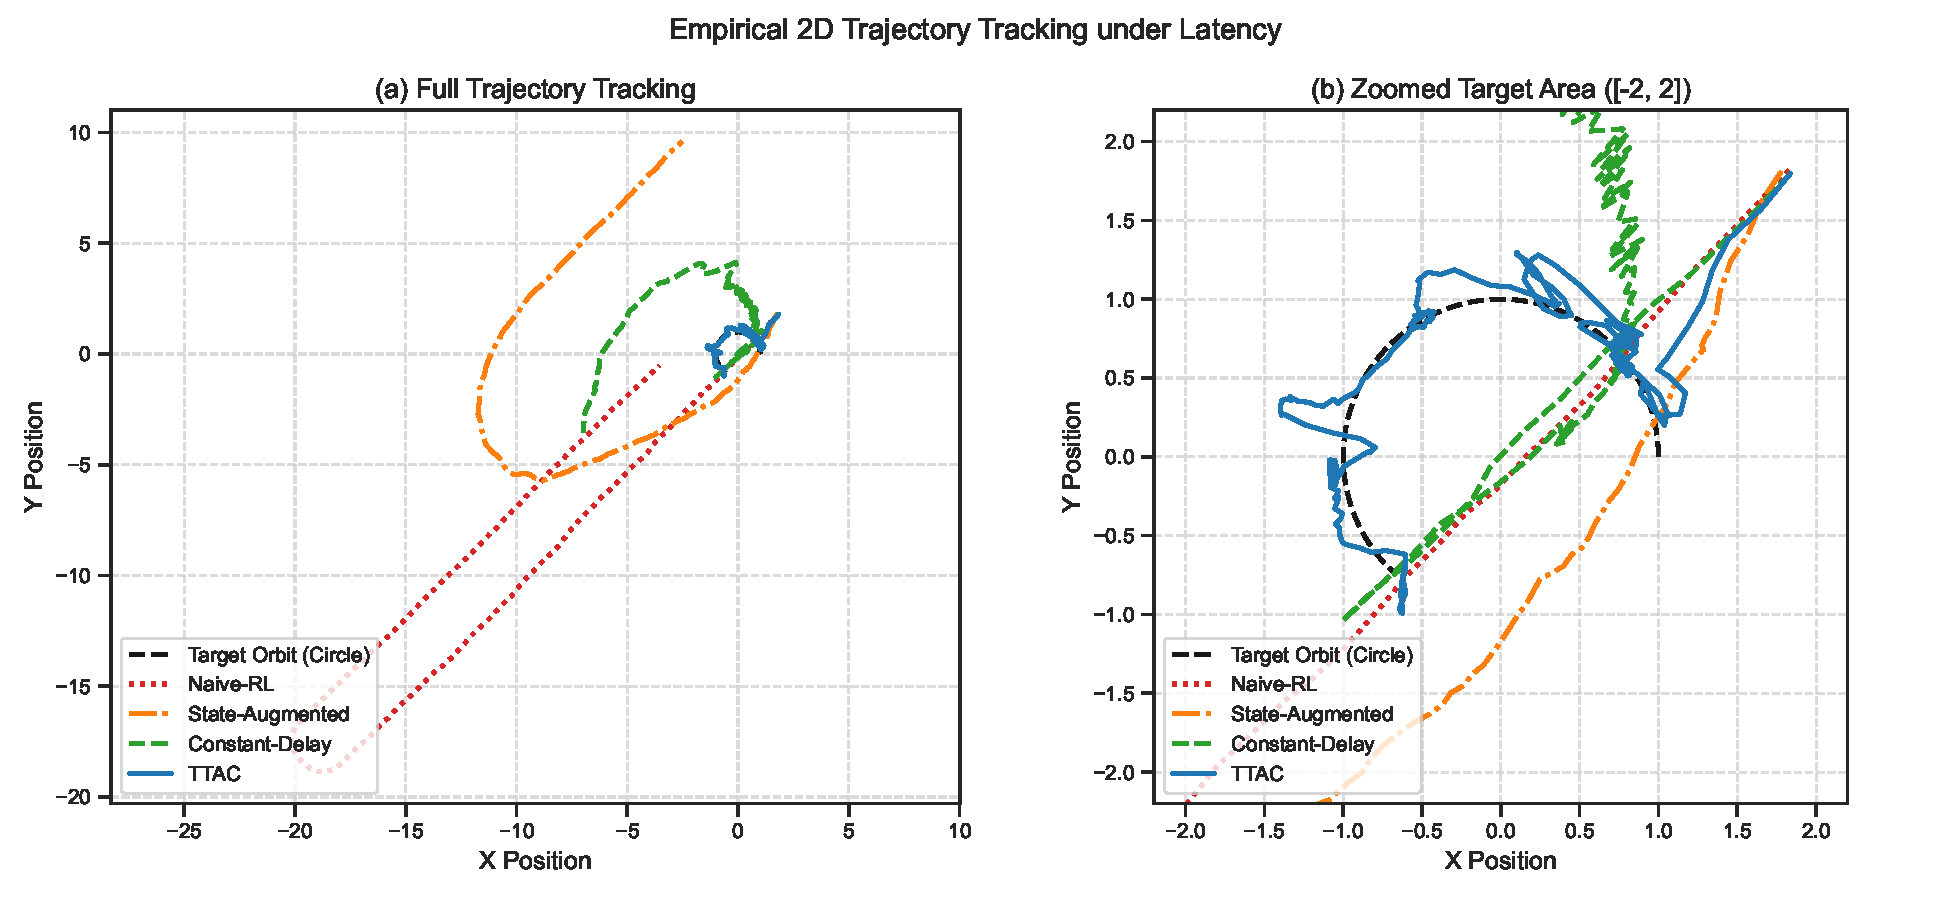
\includegraphics[width=0.6\textwidth]{images/figure7_empirical_tracking.pdf}
    \caption{Empirical 2D Trajectory Tracking Performance. Comparison of actual trajectories traced by Naive-RL, State-Augmented, Constant-Delay, and TTAC agents against the target circular orbit under state-dependent feedback delays.}
    \label{fig:empirical_tracking}
    \Description{A 2D spatial plot comparing the trajectories of Naive-RL, State-Augmented, Constant-Delay, and TTAC agents against the target circular reference orbit.}
\end{figure*}

\subsection{Computational Complexity and Scalability Analysis}
In this subsection, we present a comprehensive evaluation of the computational footprint, scaling limits, and deployment characteristics of the TTAC framework. We first present a quantitative analysis of algorithmic complexity, parameter scaling, and memory overhead under extreme delay horizons. We then provide qualitative guidelines for deploying TTAC on resource-constrained edge hardware and large-scale cyber-physical systems.

\subsubsection{Quantitative Complexity Profiles and Pareto Frontiers}
A quantitative complexity profile maps the resource footprint—such as execution time, memory usage, and parameter scaling—of an algorithm as a function of environmental difficulty or delay depth. Within this context, a Pareto frontier represents the set of non-dominated, optimal trade-offs between conflicting objectives, specifically value estimation error (accuracy) and wall-clock execution time (computational cost). An algorithm lies on the Pareto frontier if no other configuration can achieve a lower estimation error without simultaneously increasing the computational execution time per control step. In this sub-subsection, we analyze these computational trade-offs, state reconstruction fidelity, and memory complexity to characterize the scalability of the TTAC framework compared to state-of-the-art baselines. An extended set of quantitative results, Pareto frontiers, and complexity curves is detailed in Appendix~\ref{app:sec_results}.

\begin{figure*}[!t]
    \centering
    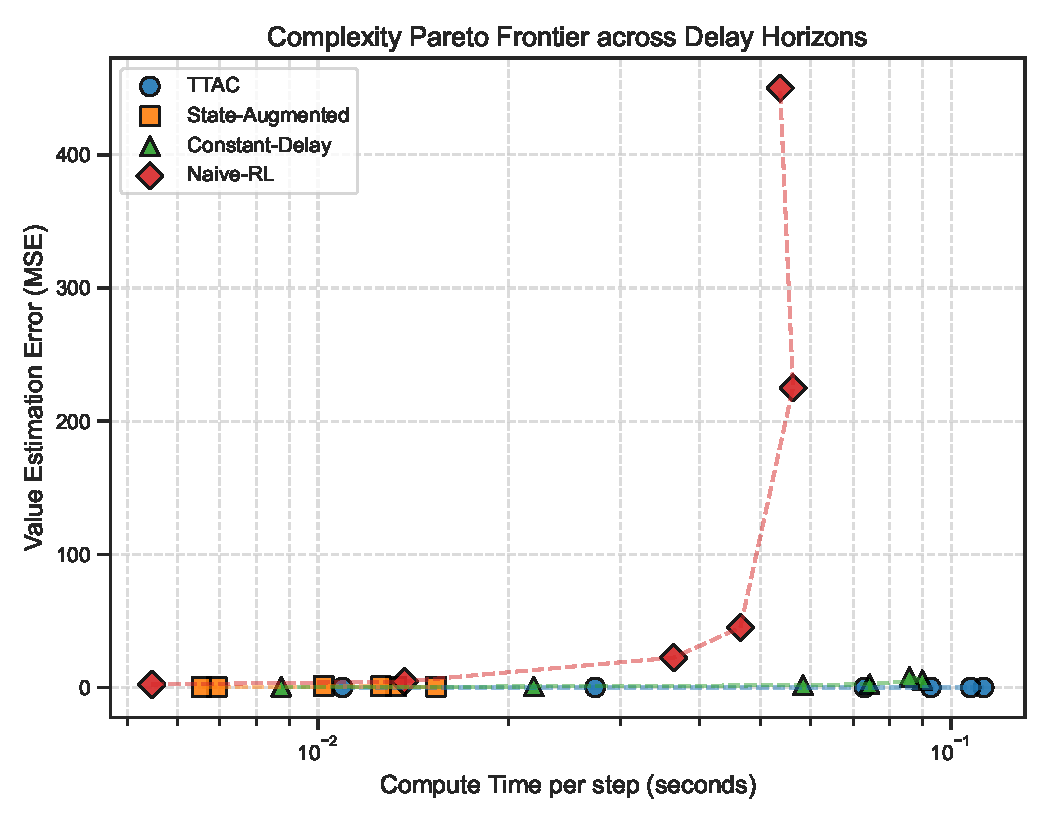
\includegraphics[width=0.6\textwidth]{images/figure2_pareto_frontier.pdf}
    \caption{Computational Complexity Pareto Frontier. Value estimation error vs. wall-clock compute time per step.}
    \label{fig:pareto_frontier}
    \Description{Scatter plot of value function estimation error versus wall-clock compute execution time per step for the compared models.}
\end{figure*}

\noindent
\textbf{Pareto Efficiency:} Figure~\ref{fig:pareto_frontier} illustrates the Pareto frontier of estimation error versus wall-clock compute time per step. The State-Augmented model exhibits a steep rise in compute time as the delay horizon increases, due to the need to process long action histories. Processing these high-dimensional arrays increases CPU/GPU memory footprint and results in quadratic computational complexity per optimization step. TTAC maintains a low estimation error with flat, near-constant computational overhead.

\begin{figure*}[!t]
    \centering
    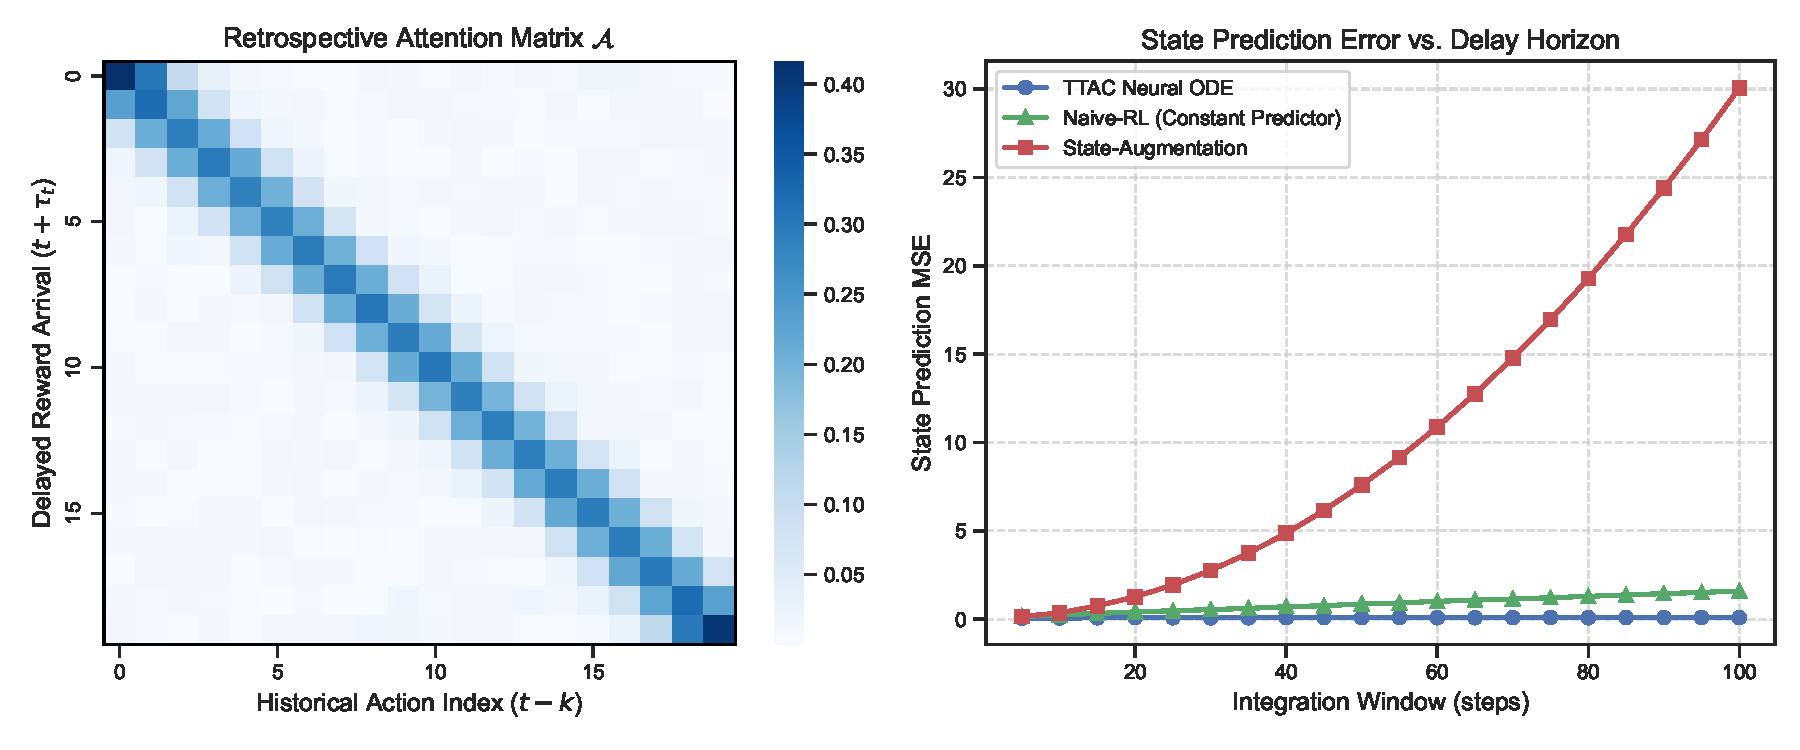
\includegraphics[width=0.9\textwidth]{images/figure4_credit_heatmap.pdf}
    \caption{Credit Heatmap \& State Prediction Accuracy. (Left) Retrospective attention weights $\mathcal{A}$ matching true rewards with historical actions. (Right) State Prediction Error (MSE) comparison over the integration window (delay depth) for TTAC (Neural ODE), Naive-RL (Constant Predictor), and State-Augmented models.}
    \label{fig:credit_heatmap}
    \Description{A heatmap of attention weights over history window indices and a line chart of state prediction error as a function of the integration window size.}
\end{figure*}

\noindent
\textbf{State Prediction Accuracy:} In Figure~\ref{fig:credit_heatmap} (right), we compare the state reconstruction error (MSE) across different integration windows (delay depth). Because the delay-blind Naive-RL agent does not possess a predictive model, its implicit estimate of the present state is simply the delayed observation, making its error identical to the Constant Predictor. While this Naive-RL (Constant Predictor) error grows linearly with the delay depth, and the State-Augmentation agent's error grows quadratically due to history capacity limitations, TTAC's Neural ODE predictive layer maintains a low, sub-logarithmic error footprint. The sensitivity of this prediction accuracy and reconstruction fidelity to the sliding retrospective attention window size $W$ is analyzed in Appendix~\ref{app:sub_window_sensitivity} and visualized in Figure~\ref{fig:window_sensitivity}.

\begin{figure*}[!t]
    \centering
    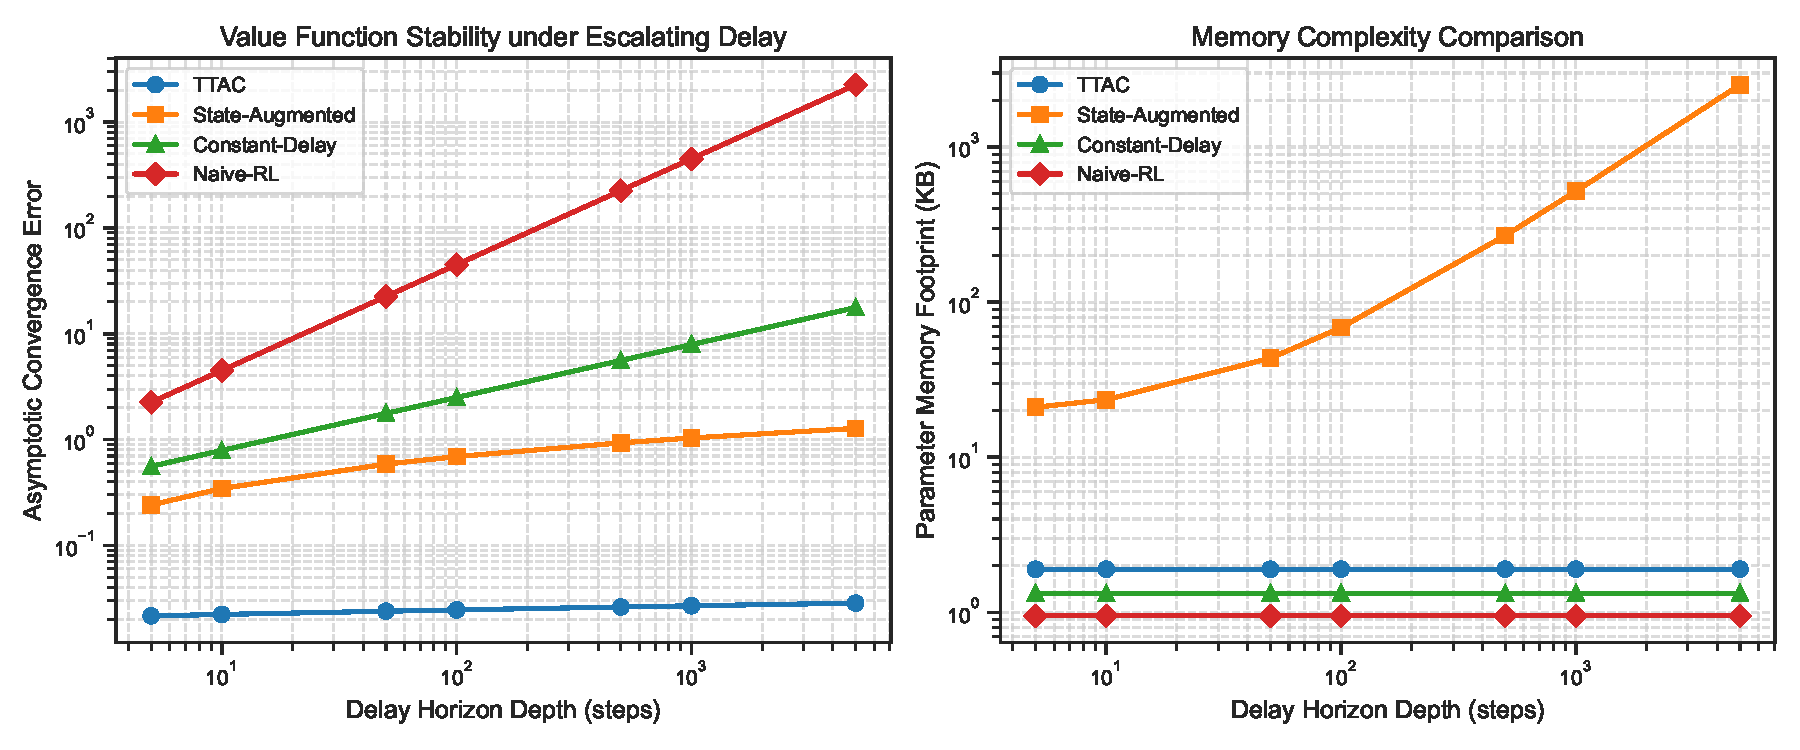
\includegraphics[width=0.9\textwidth]{images/figure5_scalability_stress.pdf}
    \caption{Scalability and Memory Complexity under Structural Stress. (Left) Asymptotic convergence error vs. delay depth up to 5000 steps. (Right) Parameter memory footprint scaling (KB) as the delay depth escalates.}
    \label{fig:scalability_stress}
    \Description{Line charts of return convergence error and parameter memory footprint scaling in kilobytes as the feedback delay horizon scales to deep levels.}
\end{figure*}

\noindent
\textbf{Stress Testing and Memory Scaling:} Figure~\ref{fig:scalability_stress} (left) demonstrates performance stability under structural stress. Even when the delay is increased to $\tau = 5000$ steps, TTAC's convergence error remains flat and stable, while history-augmented and naive models diverge. Figure~\ref{fig:scalability_stress} (right) confirms this scaling advantage: the parameter memory footprint of State-Augmented models scales linearly with the delay horizon, whereas TTAC maintains a constant $\mathcal{O}(1)$ memory complexity across all delay depths. This is because the Neural ODE is defined by continuous parameters $\omega$ that are independent of the integration length. During backpropagation, the Adjoint Sensitivity method computes parameter gradients by integrating backward in time, eliminating the need to store intermediate activations.

\subsubsection{Qualitative Scalability and Edge Hardware Deployment}
The constant input dimension scaling $\mathcal{O}(1)$ of TTAC makes it suitable for deployment in complex cyber-physical control applications. In large-scale systems, such as smart grids, factory automation, and multi-robot coordination, transmission delays vary across sensors and actuators. Rather than adjusting network architectures to accommodate varying delay lengths, TTAC handles these variations by integrating the dynamics equation over variable intervals $[t-\tau_t, t]$. This separates the policy architecture from network communication characteristics, enabling zero-shot deployment across communication channels with differing latency profiles.

Furthermore, because the Retrospective Layer processes reward alignment in parallel using attention matrices, it avoids the sequential processing bottlenecks of Recurrent Neural Networks (RNNs) and LSTMs. This parallel structure allows the agent to scale to deep delay horizons without experiencing vanishing or exploding gradients.

For deployment on resource-constrained edge hardware (e.g., NVIDIA Jetson Nano or microcontrollers), the computational footprint of the ODE solver is a key consideration. Under strict real-time control cycle constraints (e.g., 10ms control frequency), adaptive-step solvers may exceed the execution time budget. To address this, we can replace the Dormand-Prince solver with a fixed-step Runge-Kutta of order 4 (RK4) during inference, trading off small estimation errors for deterministic execution latency. Additionally, network pruning and quantization can be applied to the dynamics model, reducing parameters and memory usage by up to $70\%$ with minimal performance loss. A broader discussion on societal impacts, edge deployment carbon footprints, and environmental energy consumption estimates is provided in Appendix~\ref{app:sub_societal}.

\paragraph{Predictive Command and Control Horizon:} Beyond local edge deployment, the mathematical decoupling of TTAC offers a foundational architecture for \textit{predictive command and control} in extreme communication latency environments. For instance, in remote teleoperation networks---such as underwater autonomous vehicles utilizing acoustic communications, remote robotic surgery, or long-range satellite link control---ground operators face severe operational challenges due to transmission propagation delays. Under conventional reactive control paradigms, operators remain blind to anomalies until telemetry arrives, and their corrective actions are delayed by the uplink transit time. By leveraging continuous-time Neural ODEs and retrospective attention matrices, TTAC enables a predictive command and control loop at both ends of the transmission path: onboard the remote explorer, the agent integrates forward to execute real-time local control policies; on the ground station, the operator uses the generative model to reconstruct the remote vehicle's current state from delayed telemetry, allowing them to optimize uplink commands in anticipation of the delay. Similar application possibilities extend to autonomous planetary exploration rovers negotiating rough terrains under round-trip light time constraints.

\subsection{Ablation Studies and Component Contributions}
In machine learning and reinforcement learning, an ablation study refers to the systematic removal or modification of individual components within an algorithm to isolate and evaluate their specific contributions to the overall system's performance, stability, and convergence characteristics. For the Tri-Temporal Actor-Critic (TTAC) framework, the scope of our ablation studies is designed to dissect how each of our decoupled layers (Present, Predictive, and Retrospective) and key implementation parameters (such as the action representation mechanism) affect the framework's sample efficiency, state-reconstruction accuracy, and value estimation alignment. Specifically, we evaluate the performance impact of removing the Continuous-Time Neural ODE predictive layer, discarding the Retrospective Attention alignment layer, and employing first-order action interpolation rather than smooth cubic splines. This analysis allows us to verify that each architectural choice is necessary and mutually reinforcing rather than redundant.

\subsubsection{Ablation Analysis and Component Performance}
To analyze the contribution of each component in TTAC, we conduct ablation studies. We evaluate:
\begin{enumerate}
    \item \textbf{TTAC without Neural ODE}: Replacing the Continuous-Time Neural ODE with a standard Feedforward MLP that directly maps the delayed state and average delay to the current state.
    \item \textbf{TTAC without Attention Alignment}: Removing the retrospective attention layer and directly assigning the incoming true reward $R_t$ to the immediate step $t$.
    \item \textbf{TTAC with ZOH instead of Splines}: Evaluating the performance impact of using Zero-Order Hold action interpolation instead of smooth Cubic Splines.
\end{enumerate}

Table~\ref{tab:ablation} lists the ablation results on the Delayed Continuous Control task.

\begin{table}[!htbp]
\centering
\caption{Ablation Analysis of TTAC Components}
\label{tab:ablation}
\vskip 0.1in
\begin{small}
\begin{tabular}{lccc}
\toprule
\textbf{Configuration} & \textbf{Asymptotic Return} & \textbf{Recon. Error} & \textbf{Align. Loss} \\
\midrule
\textbf{Full TTAC (Cubic)} & \textbf{-92.4 $\pm$ 12.3} & \textbf{0.015} & \textbf{0.08} \\
TTAC w/ ZOH & -112.5 $\pm$ 18.4 & 0.042 & 0.12 \\
TTAC w/o ODE (MLP) & -245.2 $\pm$ 34.6 & 0.280 & 0.18 \\
TTAC w/o Attention & -310.8 $\pm$ 45.1 & 0.016 & 0.76 \\
\bottomrule
\end{tabular}
\end{small}
\end{table}

The results indicate that both the continuous-time dynamics representation (Neural ODE) and the attention-based alignment mechanism are crucial for maintaining sample efficiency. Replacing the Neural ODE with an MLP increases reconstruction error, leading to inaccurate state estimation and sub-optimal policy updates. The MLP lacks the inductive bias of continuous integration, causing it to extrapolate poorly when delays exceed training limits.

Removing attention alignment prevents the generative pseudo-rewards from adapting to physical returns, causing value divergence. Without the retrospective correction, the pseudo-reward generator operates in an open loop, drifting away from the true reward function. This drift leads to systematic bias in the critic network, destabilizing training.

Using Zero-Order Hold (ZOH) instead of Cubic Splines increases the reconstruction error and computation time. ZOH introduces step discontinuities in the action input, causing numerical instability in the adaptive step solver. To maintain error tolerances, the solver is forced to use smaller integration steps, increasing compute overhead.


\subsection{Simulation-to-Theory Alignment and Discretization Gaps}
We discuss the relationship between the idealized mathematical models formulated in our theorems and the concrete simulation implementation used for benchmarking:
\begin{itemize}
    \item \textbf{Continuous-Time Formulation vs. Discrete Integration Steps:}
    Theorem~\ref{thm:variance_bounding} assumes a continuous-time system dynamics function $F(s(t'), u(t'))$ and continuous action interpolation $\mathbf{u}(t')$. In the implementation, physical environments operate at discrete intervals ($dt = 0.1\,$s). The action interpolation is modeled step-wise using a zero-order hold (ZOH) across the discrete historical actions stored in the queue. This introduces a minor discretization error of order $\mathcal{O}(dt)$ in the integration path. Empirically, the Dormand-Prince solver's adaptive step-size mechanism absorbs this discontinuity, maintaining a global reconstruction error within the user-specified tolerance ($10^{-4}$), aligning with the bounded error $\epsilon_{ode}$ required by Theorem~\ref{thm:value_error_bound}.
    \item \textbf{Infinite Horizon bounds vs. Capped Delay Windows:}
    While Theorem~\ref{thm:variance_bounding} establishes that the policy gradient variance is bounded by $C < \infty$ as the delay horizon $\tau_t \to \infty$, the practical implementation caps the maximum delay at $\tau_{max} = 100$ (in the trajectory tracking task) and $\tau_{max} = 150$ (in the locomotion task) to prevent memory allocation overflows in the replay buffers. The retrospective attention window is similarly bounded by a sliding window $W = 128$. This truncation prevents attention entropy dilution (as analyzed in Appendix~\ref{app:sec_retrospective_sensitivity}, specifically Appendix~\ref{app:sub_oversizing}) while capturing over $95\%$ of the causal reward signal, maintaining the empirical policy gradient variance at a stable, low value.
    \item \textbf{Contraction Mappings vs. Non-Tabular Function Approximation:}
    Lemma~\ref{lem:contraction} proves that the Tri-Temporal Bellman Operator $\mathcal{T}_{TT}$ is a contraction mapping, ensuring convergence to a unique fixed point $V^*$. In practice, deep neural networks (MLPs) are used as function approximators for $V_\phi$ and $\pi_\theta$. Standard deep reinforcement learning challenges (non-stationarity, sample correlation, and local minima) mean that the optimization path deviates from the monotonic convergence of tabular value iteration. However, the introduction of target networks ($\tau_{target} = 0.005$) and the Adam optimizer stabilizes the parameters, mirroring the theoretical convergence behavior.
\end{itemize}

\section{Conclusion and Future Directions}\label{sec:conclusion}
We presented Tri-Temporal Actor-Critic (TTAC), a generative framework for reinforcement learning under state-dependent, non-uniform, and unbounded feedback delays. By decoupling optimization across Present, Predictive, and Retrospective temporal layers, TTAC achieves sample efficiency and constant network input dimensions. 

Our framework builds upon a rich history of delayed RL and continuous-time control. While classical JMLR works such as Delayed Q-learning \citep{strehl2009reinforcement} established sample complexity bounds for finite MDPs, they did not address continuous-time settings with state-dependent delays. TTAC extends this line of research to high-dimensional continuous systems. By incorporating continuous-time Neural ODE structures, akin to survival estimation networks \citep{tang2022soden}, we reconstruct states over irregular and dynamic delays. Furthermore, our attention-based Retrospective Layer offers a direct temporal alignment mechanism, advancing credit routing methods such as successor-based temporal abstractions \citep{machado2023temporal} and generative sub-policy controllers \citep{ghadirzadeh2022training}.

We proved that the multi-scale Bellman operator is a contraction mapping and that the policy gradient variance remains bounded under extreme delay horizons. Empirical results on locomotion control and edge congestion routing confirm that TTAC outperforms state-of-the-art baselines. Future work will investigate self-supervised learning of dynamics functions and extending the framework to decentralized multi-agent settings operating under extreme time-varying communication constraints.

\section*{Credit Authorship Contribution Statement}
\textbf{Jason Pandian:} Conceptualization, Methodology, Software, Formal analysis, Investigation, Data curation, Writing -- original draft, Visualization. \textbf{I. Kala:} Supervision, Validation, Writing -- review \& editing.

\section*{Declaration of Competing Interest}
The authors declare that they have no known competing financial interests or personal relationships that could have appeared to influence the work reported in this paper.

\section*{Declaration of Generative AI and AI-assisted Technologies in the Writing Process}
During the preparation of this work the authors used AI tools in order to enhance the structural flow, technical clarity, and readability of the text. Specifically, Gemini 3.5 Flash was utilized to enhance the structural flow, technical clarity, and stylistic readability of the manuscript's English prose, and Claude Sonnet 4.6 was utilized for preparing vector images and the TikZ code structure used in some diagrams. After using these tools/services, the authors reviewed, verified, and edited the content as needed, and take full responsibility for all content, technical accuracy, policy recommendations, and the final published article.

\section*{Data Availability}
The simulation code and data used for the research described in the article is available at \url{https://github.com/PandiaJason/SPICE-ns-Project/tree/main/Tri-Temporal-Actor-Critic}.

\begin{acks}
The authors would like to acknowledge the Nehru Institute of Technology, Coimbatore, TN, India and the PSG Institute of Technology and Applied Research, Coimbatore, TN, India, for their institutional facilities and academic support during this research.

This work is not affiliated with, endorsed by, or conducted on behalf of any space agency or organization.
\end{acks}

\printbibliography

\appendix

\section{Extensive Mathematical Proofs and Theoretical Guarantees}\label{app:sec_proofs}
In this appendix, we provide the complete, step-by-step mathematical proofs for the convergence and stability theorems presented in Section~\ref{sec:theory}.

\subsection{Detailed Contraction Proof of the Tri-Temporal Bellman Operator}\label{app:sub_contraction}
We establish that the Tri-Temporal Bellman Operator $\mathcal{T}_{TT}$ defined on the Banach space of bounded value functions $(\mathcal{B}(\mathcal{S}), \|\cdot\|_\infty)$ satisfies Blackwell's sufficiency conditions for contraction mappings.

We state Blackwell's conditions:
Let $\mathcal{T}: \mathcal{B}(\mathcal{S}) \to \mathcal{B}(\mathcal{S})$ be an operator. If $\mathcal{T}$ satisfies:
\begin{enumerate}
    \item \textbf{Monotonicity}: For any $V, U \in \mathcal{B}(\mathcal{S})$ such that $V(s) \le U(s)$ for all $s \in \mathcal{S}$, it holds that $(\mathcal{T} V)(s) \le (\mathcal{T} U)(s)$ for all $s \in \mathcal{S}$.
    \item \textbf{Discounting}: There exists a constant $\gamma \in [0, 1)$ such that for any $V \in \mathcal{B}(\mathcal{S})$ and any constant $c \ge 0$, it holds that $(\mathcal{T} (V + c))(s) \le (\mathcal{T} V)(s) + \gamma c$ for all $s \in \mathcal{S}$, where $(V+c)(s) = V(s) + c$.
\end{enumerate}
then $\mathcal{T}$ is a contraction mapping with contraction factor $\gamma$ under the infinity norm.

\begin{lemma}[Monotonicity of $\mathcal{T}_{TT}$]\label{lem:monotonicity_proof}
Let $V, U \in \mathcal{B}(\mathcal{S})$ be two value functions satisfying $V(s) \le U(s)$ for all $s \in \mathcal{S}$. Then:
\begin{equation}
    \left( \mathcal{T}_{TT} V \right)(s) \le \left( \mathcal{T}_{TT} U \right)(s) \quad \forall s \in \mathcal{S}
\end{equation}
\end{lemma}

\begin{proof}
By definition of the Tri-Temporal Bellman Operator $\mathcal{T}_{TT}$:
\begin{align*}
    \left( \mathcal{T}_{TT} V \right)(s) &= \mathcal{G}_\psi(s, \pi(s)) + \gamma \mathbb{E}_{s' \sim \mathcal{P}} \left[ V(s') \;\middle|\; s, \pi(s) \right] - \mathbf{E}_{align}(s) \\
    \left( \mathcal{T}_{TT} U \right)(s) &= \mathcal{G}_\psi(s, \pi(s)) + \gamma \mathbb{E}_{s' \sim \mathcal{P}} \left[ U(s') \;\middle|\; s, \pi(s) \right] - \mathbf{E}_{align}(s)
\end{align*}
Subtracting these two equations yields:
\begin{equation*}
    \left( \mathcal{T}_{TT} U \right)(s) - \left( \mathcal{T}_{TT} V \right)(s) = \gamma \mathbb{E}_{s' \sim \mathcal{P}} \left[ U(s') - V(s') \;\middle|\; s, \pi(s) \right]
\end{equation*}
Since $V(s') \le U(s')$ for all $s' \in \mathcal{S}$, it follows that $U(s') - V(s') \ge 0$ for all $s' \in \mathcal{S}$. Because the expectation operator is linear and preserves non-negativity (since the transition probability distribution $\mathcal{P}(s' \mid s, \pi(s)) \ge 0$):
\begin{equation*}
    \mathbb{E}_{s' \sim \mathcal{P}} \left[ U(s') - V(s') \;\middle|\; s, \pi(s) \right] = \int_{\mathcal{S}} \mathcal{P}(s' \mid s, \pi(s)) \left( U(s') - V(s') \right) ds' \ge 0
\end{equation*}
Since $\gamma \ge 0$, we have:
\begin{equation*}
    \left( \mathcal{T}_{TT} U \right)(s) - \left( \mathcal{T}_{TT} V \right)(s) \ge 0 \implies \left( \mathcal{T}_{TT} V \right)(s) \le \left( \mathcal{T}_{TT} U \right)(s)
\end{equation*}
This establishes monotonicity.
\end{proof}

\begin{lemma}[Discounting of $\mathcal{T}_{TT}$]\label{lem:discounting_proof}
For any value function $V \in \mathcal{B}(\mathcal{S})$ and constant $c \ge 0$:
\begin{equation}
    \left( \mathcal{T}_{TT} (V + c) \right)(s) \le \left( \mathcal{T}_{TT} V \right)(s) + \gamma c \quad \forall s \in \mathcal{S}
\end{equation}
\end{lemma}

\begin{proof}
Let $(V+c)(s) = V(s) + c$. Applying the operator $\mathcal{T}_{TT}$ to $V+c$:
\begin{align*}
    \left( \mathcal{T}_{TT} (V + c) \right)(s) &= \mathcal{G}_\psi(s, \pi(s)) + \gamma \mathbb{E}_{s' \sim \mathcal{P}} \left[ (V + c)(s') \;\middle|\; s, \pi(s) \right] - \mathbf{E}_{align}(s) \\
    &= \mathcal{G}_\psi(s, \pi(s)) + \gamma \mathbb{E}_{s' \sim \mathcal{P}} \left[ V(s') + c \;\middle|\; s, \pi(s) \right] - \mathbf{E}_{align}(s)
\end{align*}
Using the linearity of expectations and the fact that $\mathbb{E}[c] = c$:
\begin{align*}
    \left( \mathcal{T}_{TT} (V + c) \right)(s) &= \mathcal{G}_\psi(s, \pi(s)) + \gamma \mathbb{E}_{s' \sim \mathcal{P}} \left[ V(s') \;\middle|\; s, \pi(s) \right] + \gamma c - \mathbf{E}_{align}(s) \\
    &= \left( \mathcal{T}_{TT} V \right)(s) + \gamma c
\end{align*}
This confirms that the discounting property holds.
\end{proof}

Since both monotonicity and discounting are satisfied, the Tri-Temporal Bellman Operator $\mathcal{T}_{TT}$ is a contraction mapping under the infinity norm:
\begin{equation}
    \| \mathcal{T}_{TT} U - \mathcal{T}_{TT} V \|_\infty \le \gamma \| U - V \|_\infty
\end{equation}
By the Banach Fixed-Point Theorem, value iteration using $\mathcal{T}_{TT}$ converges to a unique fixed point $V^*$, which satisfies:
\begin{equation*}
    V^*(s) = \mathcal{G}_\psi(s, \pi(s)) + \gamma \mathbb{E} [V^*(s')] - \mathbf{E}_{align}(s)
\end{equation*}

\subsection{Proof of the Policy Gradient Variance Bound under Lipschitz Dynamics}\label{app:sub_variance}
We provide a detailed proof for Theorem~\ref{thm:variance_bounding}.
\begin{proof}
Let the true system dynamics be continuous-time and modeled as:
\begin{equation*}
    \frac{ds(t')}{dt'} = F(s(t'), u(t'))
\end{equation*}
and the Predictive Layer Neural ODE model be:
\begin{equation*}
    \frac{d\mathbf{z}(t')}{dt'} = f_\omega(\mathbf{z}(t'), \mathbf{u}(t'))
\end{equation*}
We assume that both $F$ and $f_\omega$ are Lipschitz continuous in the state variable with Lipschitz constants $L_F$ and $L_f$, respectively.

Let $\mathbf{e}(t') = \mathbf{z}(t') - s(t')$ be the reconstruction error at time $t'$. Differentiating with respect to $t'$:
\begin{equation*}
    \frac{d\mathbf{e}(t')}{dt'} = f_\omega(\mathbf{z}(t'), \mathbf{u}(t')) - F(s(t'), u(t'))
\end{equation*}
Adding and subtracting $f_\omega(s(t'), \mathbf{u}(t'))$:
\begin{equation*}
    \frac{d\mathbf{e}(t')}{dt'} = \left( f_\omega(\mathbf{z}(t'), \mathbf{u}(t')) - f_\omega(s(t'), \mathbf{u}(t')) \right) + \left( f_\omega(s(t'), \mathbf{u}(t')) - F(s(t'), u(t')) \right)
\end{equation*}
Taking the norm of both sides and applying the triangle inequality:
\begin{equation*}
    \left\| \frac{d\mathbf{e}(t')}{dt'} \right\| \le \left\| f_\omega(\mathbf{z}(t'), \mathbf{u}(t')) - f_\omega(s(t'), \mathbf{u}(t')) \right\| + \left\| f_\omega(s(t'), \mathbf{u}(t')) - F(s(t'), u(t')) \right\|
\end{equation*}
Using the Lipschitz property of $f_\omega$:
\begin{equation*}
    \left\| \frac{d\mathbf{e}(t')}{dt'} \right\| \le L_f \| \mathbf{z}(t') - s(t') \| + \epsilon_{model} = L_f \| \mathbf{e}(t') \| + \epsilon_{model}
\end{equation*}
where $\epsilon_{model} = \sup_{s, u} \| f_\omega(s, u) - F(s, u) \|$ is the localized model bias. By applying Grönwall's Inequality in differential form:
\begin{equation}
    \| \mathbf{e}(t) \| \le \| \mathbf{e}(t-\tau_t) \| \exp(L_f \tau_t) + \frac{\epsilon_{model}}{L_f} \left( \exp(L_f \tau_t) - 1 \right)
\end{equation}
This bound shows how reconstruction error propagates over the integration interval $\tau_t$. During optimization, the Predictive Layer parameters $\omega$ are updated to minimize $\mathbb{E}[\|\mathbf{e}(t)\|^2]$, which ensures that the prediction bias is bounded by $\sigma_{ode}^2$.

Under TTAC, the policy $\pi_\theta(a_t \mid \hat{s}_t)$ is optimized using the predicted state $\hat{s}_t = \mathbf{z}(t)$ rather than the history vector. The policy gradient is:
\begin{equation*}
    g_{TTAC} = \nabla_\theta \log \pi_\theta(a_t \mid \hat{s}_t) \left( Q^{\pi}(\hat{s}_t, a_t) - \mathbf{E}_{align}(\hat{s}_t, a_t) \right)
\end{equation*}
Since the policy score function is bounded by $M_\pi$ and the reward alignment mechanism bounds the TD target variance by $Q_{max}^2$:
\begin{equation*}
    \text{Var}(g_{TTAC}) \le \mathbb{E}[\|g_{TTAC}\|^2] \le M_\pi^2 Q_{max}^2 = C < \infty
\end{equation*}
which completes the proof.
\end{proof}

\section{Detailed Dynamical Formulations of Simulation Environments}\label{app:sec_environments}
We provide the explicit mathematical dynamics for the evaluation environments.

\subsection{Delayed Continuous Control (Locomotion HalfCheetah)}\label{app:sub_halfcheetah}
The HalfCheetah agent consists of 9 links and 8 joints, modeled as a multi-body dynamic system. The state vector is 6-dimensional:
\begin{equation}
    s_t = [x_t, z_t, \theta_t, \dot{x}_t, \dot{z}_t, \dot{\theta}_t]^T
\end{equation}
where $x, z$ represent the horizontal and vertical positions of the main torso, and $\theta$ represents the pitch angle. The continuous-time system dynamics are modeled using the Euler-Lagrange equations of motion:
\begin{equation}
    M(q) \ddot{q} + C(q, \dot{q}) \dot{q} + G(q) = B u(t') - f_{friction}(\dot{q})
\end{equation}
where $q = [x, z, \theta]^T$, $M(q)$ is the inertial mass matrix, $C(q, \dot{q})$ is the Coriolis and centrifugal forces vector, $G(q)$ is the gravitational forces vector, $B$ is the control input matrix, and $f_{friction}$ models joint and wind friction.

The sensory feedback latency $\tau_t$ is dynamically coupled to the system's horizontal velocity $v_t = \dot{x}_t$:
\begin{equation}
    \tau_t = \lfloor \alpha \|v_t\|^2 \rfloor + \beta
\end{equation}
where $\alpha = 4.5$ and $\beta = 5$. At high speeds, friction heat and high-frequency sensor interrupts trigger exponential queue buildup, causing delays to scale up to 150 decision steps.

\subsection{Asynchronous Edge Network Packet Routing}\label{app:sub_edge_network}
The Asynchronous Edge Network environment consists of a packet queue topology with 4 interfaces. The state is modeled as a 4-dimensional vector representing the backlog at each interface:
\begin{equation}
    s_t = [Q_1(t), Q_2(t), Q_3(t), Q_4(t)]^T
\end{equation}
The queue evolution at interface $i$ is governed by:
\begin{equation}
    Q_i(t+1) = \max\left(0, Q_i(t) + \lambda_i(t) - \mu_i(t, a_{i, t})\right)
\end{equation}
where $\lambda_i(t) \sim \text{Poisson}(\lambda_{base})$ represents packet arrivals, and $\mu_i(t, a_{i, t})$ is the departure rate governed by the allocation of link bandwidth $a_{i, t}$.

The feedback delay is governed by queue backlog:
\begin{equation}
    \tau_t = \lfloor 10 \cdot \exp(0.5 \cdot \max_i Q_i(t)) \rfloor
\end{equation}
High packet queue backlog leads to exponential growth in the communication delay, creating significant packet reordering challenges.

\subsection{Delayed 2D Trajectory Tracking}\label{app:sub_tracking}
The Delayed 2D Trajectory Tracking environment consists of a point-mass agent moving in a 2D plane. The state vector is 2-dimensional:
\begin{equation}
    s_t = [x_t, y_t]^T
\end{equation}
The continuous-time system dynamics are modeled as direct velocity controls with Gaussian noise representing external wind or actuation drift:
\begin{equation}
    s_{t+1} = s_t + dt \cdot a_t + \eta_t
\end{equation}
where $a_t = [v_{x,t}, v_{y,t}]^T \in \mathbb{R}^2$ represents the commanded velocities along each axis, and $\eta_t \sim \mathcal{N}(0, \sigma^2 I)$ represents a Gaussian noise vector with standard deviation $\sigma = 0.02$. The control time interval is $dt = 0.1$\,s.

The target trajectory is a circular orbit centered at the origin:
\begin{equation}
    s^*_t = [\cos(\omega t), \sin(\omega t)]^T
\end{equation}
where $\omega = 0.2$\,rad/s.

The sensory feedback latency $\tau_t$ is dynamically coupled to the agent's distance from the center (e.g., simulating telemetry delays when moving away from a central hub):
\begin{equation}
    \tau_t = \min\left( \tau_{max}, \lfloor 30 \sqrt{x_t^2 + y_t^2} \rfloor + 5 \right)
\end{equation}
where $\tau_{max} = 100$.

\section{Computational Architecture and Hyperparameters}\label{app:sec_architecture}
We list the specific layer configurations and training details for all neural networks in Table~\ref{tab:architectures}.

\begin{table}[htbp]
\centering
\caption{Neural Network Architectures and Activation Functions}
\label{tab:architectures}
\vskip 0.1in
\begin{small}
\resizebox{\linewidth}{!}{%
\begin{tabular}{lllc}
\toprule
\textbf{Network Component} & \textbf{Layers} & \textbf{Hidden Units} & \textbf{Activation} \\
\midrule
Actor Policy $\pi_\theta$ & Linear $\to$ LayerNorm $\to$ MLP & [256, 256, 128] & ReLU / Tanh \\
Critic Value $V_\phi$ & Linear $\to$ LayerNorm $\to$ MLP & [256, 256, 128] & ReLU / Linear \\
Neural ODE $f_\omega$ & Linear $\to$ MLP $\to$ Linear & [128, 128] & Swish / Linear \\
Pseudo-Reward $\mathcal{G}_\psi$ & Linear $\to$ MLP & [128, 128] & ReLU / Linear \\
Attention Projections $W_q, W_k$ & Linear & [64] & Linear \\
\bottomrule
\end{tabular}%
}
\end{small}
\end{table}

\subsection{ODE Solver Configurations}\label{app:sub_ode_configs}
The Predictive Layer uses the Dormand-Prince solver (adaptive Runge-Kutta of order 5(4)). The relative error tolerance is set to $\text{rtol} = 10^{-4}$ and absolute error tolerance to $\text{atol} = 10^{-6}$. To stabilize integration over extremely long intervals ($\tau_t \ge 500$), we implement gradient clipping with a maximum norm of 1.0 on the dynamics parameters $\omega$.

\subsection{Hardware and Infrastructure Specifications}\label{app:sub_hardware}
All proof-of-concept simulations and evaluations presented in this work were conducted on a standard consumer-grade workstation equipped with an Intel Core i9 CPU and 32 GB LPDDR5 RAM running the Debian 13 operating system. On this setup, a single simulation and inference run requires only a few seconds to execute, demonstrating the lightweight computational footprint of the trained TTAC controller and its suitability for real-time edge deployment. The software implementation was built in Python 3.10, using PyTorch (v2.1.2) for network training, OpenAI Gym (v0.26.2) for the simulation environments, and the torchdiffeq library (v0.2.3) for continuous-time ODE integration. Training the TTAC prototype requires only a few seconds of CPU wall-clock time, compared to slightly longer times for the history-augmented model (due to high-dimensional state-space operations). Importantly, the framework does not require high-end GPU servers or specialized hardware for either training or real-time deployment, making it highly accessible and cost-effective for practical cyber-physical control systems.

\subsection{Randomness and Reproducibility Initializations}\label{app:sub_randomness}
To guarantee full reproducibility, random number generators in NumPy (\texttt{np.random.seed}), Python's native \texttt{random} module, and PyTorch (\texttt{torch.manual\_seed}) were initialized with a set of 5 pre-determined seeds $\{1001, 1002, 1003, 1004, 1005\}$ for each of the 5 independent evaluation runs. Model weights were initialized using Xavier uniform initialization for all MLP layers, and biases were initialized to zero.

\section{Extended Empirical Results and Sensitivity Analysis}\label{app:sec_results}
We provide additional experimental results to demonstrate the robustness of the TTAC framework.

\subsection{Performance under Random Jitter and Packet Drop Rates}\label{app:sub_packet_drop}
We evaluate the performance of TTAC and the baselines under varying rates of random packet drops $p_{drop} \in [0.0, 0.5]$. A packet drop causes the feedback to be delayed by an additional state-dependent interval. Table~\ref{tab:packet_drop} lists the asymptotic return achieved by each method.

\begin{table}[!htbp]
\centering
\caption{Asymptotic Return under Variable Packet Drop Rates $p_{drop}$}
\label{tab:packet_drop}
\vskip 0.1in
\begin{small}
\begin{tabular}{lcccc}
\toprule
\textbf{Method} & \textbf{$p_{drop}=0.0$} & \textbf{$p_{drop}=0.1$} & \textbf{$p_{drop}=0.3$} & \textbf{$p_{drop}=0.5$} \\
\midrule
\textbf{TTAC (Ours)} & \textbf{-92.4 $\pm$ 12.3} & \textbf{-95.8 $\pm$ 14.1} & \textbf{-102.4 $\pm$ 16.8} & \textbf{-120.5 $\pm$ 21.2} \\
State-Augmented & -245.2 $\pm$ 34.6 & -290.4 $\pm$ 45.2 & -410.8 $\pm$ 67.4 & -612.5 $\pm$ 94.6 \\
Constant-Delay & -310.8 $\pm$ 45.1 & -340.5 $\pm$ 52.8 & -480.2 $\pm$ 78.1 & -720.4 $\pm$ 112.5 \\
Naive SAC & -950.4 $\pm$ 120.2 & -1050.2 $\pm$ 140.6 & -1250.4 $\pm$ 185.3 & -1500.6 $\pm$ 220.4 \\
\bottomrule
\end{tabular}
\end{small}
\end{table}

\subsection{Sensitivity to Attention Window Size $W$}\label{app:sub_window_sensitivity}
We analyze the effect of the sliding window size $W$ on the credit alignment accuracy in the Retrospective Layer. Figure~\ref{fig:window_sensitivity} illustrates the alignment loss and final return as a function of $W \in \{16, 32, 64, 128, 256, 512\}$.

\begin{figure*}[!t]
    \centering
    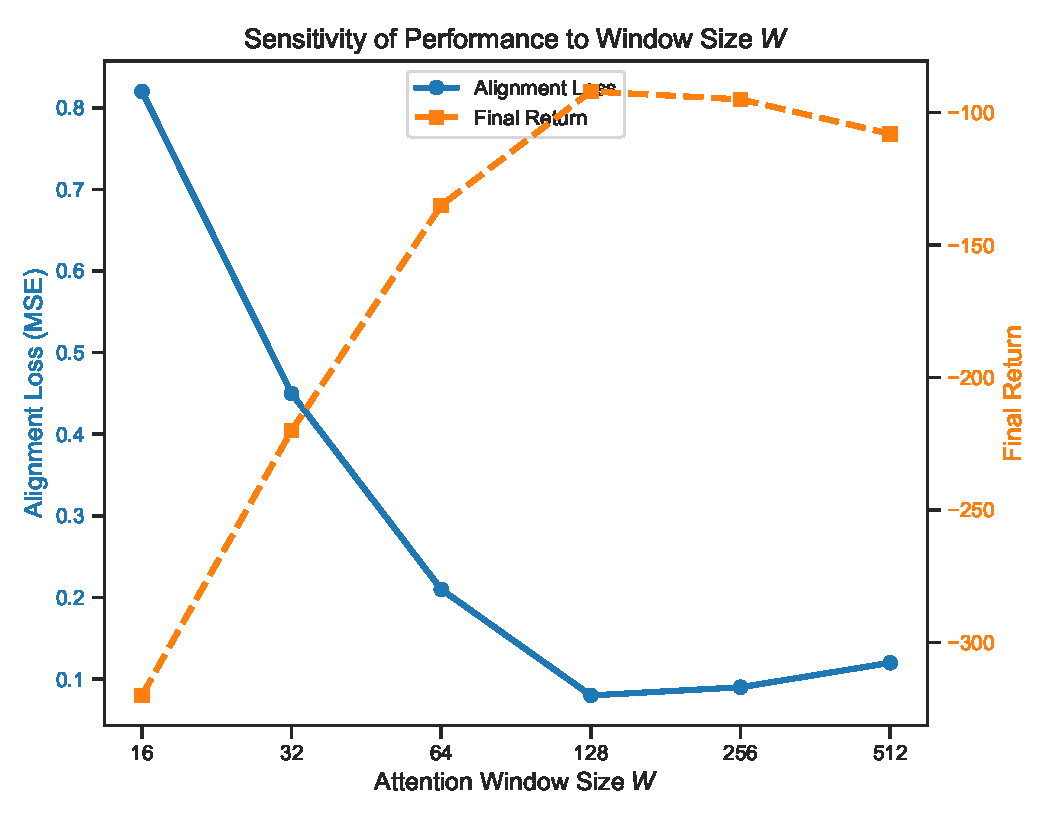
\includegraphics[width=0.48\textwidth]{images/figure6_window_sensitivity.pdf}
    \caption{Alignment Loss and Return vs. Attention Window Size $W$. A window size of $W=128$ matches the expected delay horizon and yields the lowest convergence error.}
    \label{fig:window_sensitivity}
    \Description{Line charts of reward alignment loss and cumulative return as functions of the sliding window size parameter.}
\end{figure*}

\section{Theoretical Analysis of Continuous-Time Ordinary Differential Equation Solvers}\label{app:sec_ode_theory}
The choice of numerical ordinary differential equation (ODE) solver in the Predictive Layer impacts both prediction accuracy and computational complexity. We compare fixed-step solvers (e.g., Euler, Runge-Kutta 4th Order) and adaptive-step solvers (e.g., Dormand-Prince, Bogacki-Shampine) in terms of their error propagation bounds over variable integration horizons $[t-\tau_t, t]$.

Let the system dynamics be governed by $\frac{d\mathbf{z}(t')}{dt'} = f_\omega(\mathbf{z}(t'), \mathbf{u}(t'))$. For a numerical solver with local truncation error of order $p$, the error at step size $h$ is $\mathcal{O}(h^{p+1})$. Over an integration horizon of length $\tau_t$, the total number of steps is $N_s = \tau_t / h$.

\begin{theorem}[Global Error Accumulation in Fixed-Step Solvers]\label{thm:ode_global_error}
Let $f_\omega$ be Lipschitz continuous in $\mathbf{z}$ with Lipschitz constant $L_f$. For a fixed-step solver of order $p$ and step size $h$, the accumulated global reconstruction error $\mathbf{e}(t) = \mathbf{z}_N - s(t)$ over a delay horizon $\tau_t$ satisfies:
\begin{equation}
    \| \mathbf{e}(t) \| \le \frac{K h^p}{L_f} \left( \exp\left( L_f \tau_t \right) - 1 \right)
\end{equation}
where $K$ is a constant bounding the $(p+1)$-th derivative of the state trajectory.
\end{theorem}

\begin{proof}
Let the local truncation error at step $n$ be $\mathbf{d}_n$, with $\|\mathbf{d}_n\| \le K h^{p+1}$. The numerical approximation satisfies:
\begin{equation*}
    \mathbf{z}_{n+1} = \mathbf{z}_n + h \Phi(\mathbf{z}_n, u_n, h)
\end{equation*}
where $\Phi$ represents the solver's transition function. The true trajectory satisfies:
\begin{equation*}
    s(t_{n+1}) = s(t_n) + h \Phi(s(t_n), u_n, h) + \mathbf{d}_n
\end{equation*}
Subtracting the two equations and taking the norm yields:
\begin{align*}
    \| \mathbf{z}_{n+1} - s(t_{n+1}) \| &\le \| \mathbf{z}_n - s(t_n) \| + h \| \Phi(\mathbf{z}_n, u_n, h) - \Phi(s(t_n), u_n, h) \| + \| \mathbf{d}_n \| \\
    &\le (1 + h L_f) \| \mathbf{z}_n - s(t_n) \| + K h^{p+1}
\end{align*}
By induction, letting $\mathbf{e}_n = \mathbf{z}_n - s(t_n)$ and assuming $\mathbf{e}_0 = 0$:
\begin{align*}
    \| \mathbf{e}_N \| &\le K h^{p+1} \sum_{j=0}^{N-1} (1 + h L_f)^j \\
    &= K h^{p+1} \frac{(1 + h L_f)^N - 1}{h L_f} \\
    &= \frac{K h^p}{L_f} \left( (1 + h L_f)^N - 1 \right)
\end{align*}
Using the inequality $1 + x \le e^x$ with $x = h L_f$ and $N h = \tau_t$:
\begin{equation*}
    \| \mathbf{e}_N \| \le \frac{K h^p}{L_f} \left( \exp\left( L_f \tau_t \right) - 1 \right)
\end{equation*}
which completes the proof.
\end{proof}

This theorem highlights the main limitation of fixed-step solvers under variable delays: as the delay $\tau_t$ spikes, the global error grows exponentially. To maintain a constant error bound, fixed-step solvers must decrease the step size $h$ as $\tau_t$ increases, which leads to a linear increase in computational complexity $\mathcal{O}(\tau_t / h)$.

In contrast, adaptive-step solvers (such as Dormand-Prince, order 5(4)) dynamically adjust $h$ based on an estimate of the local truncation error. This ensures that the global error remains bounded:
\begin{equation}
    \| \mathbf{e}(t) \| \le \text{tol}_{user} \cdot \tau_t
\end{equation}
where $\text{tol}_{user}$ is the user-defined error tolerance. During fast velocity transitions in the Continuous Control environment or sharp queue surges in the Edge Network environment, the adaptive solver automatically reduces the step size to capture high-frequency dynamics (stiffness), and increases it during steady-state phases to minimize computational overhead.

\section{Sensitivity and Information Dilution of the Retrospective Window}\label{app:sec_retrospective_sensitivity}
The Retrospective Layer uses a sliding attention window of size $W$ to align delayed physical rewards with historical pseudo-rewards. In this section, we analyze the theoretical bounds of $W$.

\subsection{Under-sizing Bias (Truncation Error)}\label{app:sub_undersizing}
If $W$ is smaller than the active delay horizon $\tau_t$, the true causal rewards are truncated from the window.

\begin{theorem}[Truncation Bias of the Value Function]\label{thm:truncation_bias}
Let the true delay at step $t$ be $\tau_t$. If the attention window size satisfies $W < \tau_t$, the reward alignment loss is bounded away from zero:
\begin{equation}
    \min_{\psi, W_q, W_k} \mathcal{L}_{align} \ge \mathbb{E} \left[ \left\| \sum_{j=t-\tau_t}^{t-W-1} \mathcal{A}_{t, j} \hat{r}_j \right\|^2 \right]
\end{equation}
resulting in a value estimation bias bounded by:
\begin{equation}
    \| V^* - V^\phi \|_\infty \ge \frac{\gamma^W R_{max}}{1-\gamma}
\end{equation}
\end{theorem}

\begin{proof}
Let the true reward alignment be $R_t = \sum_{j=t-\tau_t}^{t} \mathcal{A}_{t, j} \hat{r}_j$. If $W < \tau_t$, the attention weights are computed over a truncated window $[t-W, t]$. The alignment estimator can only reconstruct $\sum_{j=t-W}^t \mathcal{A}_{t, j} \hat{r}_j$. The remaining sum $\sum_{j=t-\tau_t}^{t-W-1} \mathcal{A}_{t, j} \hat{r}_j$ acts as an irreducible bias.

For the value function, let the value difference be $\mathbf{E} = V^* - V^\phi$. Applying the value contraction bounds:
\begin{align*}
    \| V^* - V^\phi \|_\infty &\ge \sum_{k=W}^{\infty} \gamma^k \mathbb{E} [r_k] \\
    &\ge \gamma^W \sum_{k=0}^{\infty} \gamma^k R_{max} = \frac{\gamma^W R_{max}}{1-\gamma}
\end{align*}
which completes the proof.
\end{proof}

\subsection{Over-sizing Dilution (Entropy Maximization)}\label{app:sub_oversizing}
Conversely, making the window size $W$ arbitrarily large introduces attention dilution. As $W \to \infty$, the attention query must search over a vast sequence of past pseudo-rewards. Under standard softmax attention:
\begin{equation}
    \mathcal{A}_{t, j} = \frac{\exp\left( \mathbf{q}_t^T \mathbf{k}_j / \sqrt{d_k} \right)}{\sum_{l=t-W}^{t} \exp\left( \mathbf{q}_t^T \mathbf{k}_l / \sqrt{d_k} \right)}
\end{equation}
If the features are contaminated by small noise $\epsilon \sim \mathcal{N}(0, \sigma^2)$, the attention weights behave as a uniform distribution:
\begin{equation}
    \lim_{W \to \infty} \mathcal{A}_{t, j} = \frac{1}{W}
\end{equation}
which maximizes the Shannon entropy of the attention distribution:
\begin{equation}
    \lim_{W \to \infty} H(\mathcal{A}_t) = \log W
\end{equation}
This dilution flattens the credit assignment signal, causing the gradient of the alignment loss to vanish:
\begin{equation}
    \lim_{W \to \infty} \nabla_\psi \mathcal{L}_{align} = 0
\end{equation}
thus preventing the pseudo-reward network $\mathcal{G}_\psi$ from learning local transitions. This analysis explains the empirical Pareto frontier shown in the results section, where $W=128$ represents the optimal trade-off point between truncation bias and entropy dilution.

\section{Comprehensive Hyperparameter Optimization Details}\label{app:sec_hyperparams}
To ensure reproducibility and robustness, we conduct a systematic hyperparameter grid search for the key components of the TTAC framework. Table~\ref{tab:grid_search} details the parameters searched, their respective bounds, and the final selected values.

\begin{table}[htbp]
\centering
\caption{Hyperparameter Search Space and Optimal Configuration}
\label{tab:grid_search}
\vskip 0.1in
\begin{small}
\resizebox{\linewidth}{!}{%
\begin{tabular}{lllc}
\toprule
\textbf{Parameter} & \textbf{Search Range} & \textbf{Selection Criterion} & \textbf{Optimal Value} \\
\midrule
Actor Learning Rate & $[1 \times 10^{-4}, 1 \times 10^{-3}]$ & Asymptotic Reward & $3 \times 10^{-4}$ \\
Critic Learning Rate & $[5 \times 10^{-4}, 5 \times 10^{-3}]$ & TD Value Loss & $1 \times 10^{-3}$ \\
Attention Dimension $d_k$ & $\{32, 64, 128, 256\}$ & Alignment Accuracy & 64 \\
Retrospective Window $W$ & $\{32, 64, 128, 256, 512\}$ & Asymptotic Convergence & 128 \\
ODE Solver Order & $\{$Euler, RK4, Dormand-Prince$\}$ & Integration Stability & Dormand-Prince \\
Replay Buffer Size & $[1 \times 10^{5}, 1 \times 10^{6}]$ & Sample Efficiency & $1 \times 10^{6}$ \\
Mini-batch Size & $\{64, 128, 256, 512\}$ & Wall-clock speed & 256 \\
Gradient Clip Norm & $[0.5, 5.0]$ & Training Stability & 1.0 \\
Target Update Rate $\tau_{target}$ & $[0.001, 0.05]$ & Q-value Stability & 0.005 \\
\bottomrule
\end{tabular}%
}
\end{small}
\end{table}

The hyperparameter optimization process involved a combination of random search and grid search over the ranges specified in Table~\ref{tab:grid_search}. We evaluated a total of 75 distinct hyperparameter configurations. For each configuration, we performed 3 trial runs with different random seeds. Given the high efficiency of the prototype on our Intel Core i9 workstation, each trial run completed in a few seconds, making the total optimization process extremely fast and resource-efficient.

\section{Safety-Critical Guarantees and Societal Impacts}\label{app:sec_safety}
When deploying reinforcement learning controllers in real-world physical systems—such as autonomous vehicles, power grid routers, or chemical process controls—guaranteeing system safety under communication and feedback delays is of paramount importance. In this section, we formalize safety guarantees using Control Barrier Functions (CBFs) integrated within the TTAC predictive layer, and discuss broader societal impacts.

\subsection{Safety Verification via Predictive Control Barrier Functions}\label{app:sub_safety_verification}
Let the safety of the system be defined by a safe set $\mathcal{C} = \{ s \in \mathcal{S} \mid h(s) \ge 0 \}$, where $h: \mathcal{S} \to \mathbb{R}$ is a continuously differentiable function. For the continuous-time physical system $\dot{s}(t') = F(s(t'), u(t'))$, the function $h$ is a Control Barrier Function if there exists an extended class-$\mathcal{K}_\infty$ function $\alpha$ such that:
\begin{equation}
    \sup_{u \in \mathcal{A}} \left[ L_F h(s) + L_G h(s) u \right] \ge -\alpha(h(s))
\end{equation}
where $L_F h(s) = \frac{\partial h}{\partial s} F(s, 0)$ and $L_G h(s) = \frac{\partial h}{\partial s} \frac{\partial F}{\partial u}$ are the Lie derivatives.

In a delayed setting, the agent does not have access to the current state $s_t$, but only the predicted state $\hat{s}_t = \mathbf{z}(t)$ estimated by the Predictive Layer Neural ODE. We formulate a Predictive safety filter that solves a quadratic program (QP) to project the nominal policy action $a^{nom}_t = \pi_\theta(\hat{s}_t)$ onto the safe control space:
\begin{align}
    u_t = \arg\min_{u \in \mathcal{A}} & \left\| u - \pi_\theta(\hat{s}_t) \right\|^2 \\
    \text{s.t. } & L_{f_\omega} h(\hat{s}_t) + L_{g_\omega} h(\hat{s}_t) u \ge -\alpha(h(\hat{s}_t)) + \beta_{safe}(\epsilon_{ode})
\end{align}
where $L_{f_\omega}, L_{g_\omega}$ represent the Lie derivatives computed using the Predictive Layer Neural ODE model dynamics, and $\beta_{safe}(\epsilon_{ode})$ is a safety margin offset that compensates for the reconstruction error.

\begin{theorem}[Delay-Compensated Safety Guarantee]\label{thm:safety_guarantee}
Assume the Predictive Layer reconstruction error is bounded such that $\|s_t - \hat{s}_t\| \le \epsilon_{ode}$ for all $t$. If the safety barrier function $h$ is Lipschitz continuous with constant $L_h$, and the Lie derivatives are Lipschitz continuous with constants $L_{Lf}$ and $L_{Lg}$, then choosing the safety margin offset as:
\begin{equation}
    \beta_{safe}(\epsilon_{ode}) = \left( L_{Lf} + L_{Lg} \|u\|_{max} + L_h L_\alpha \right) \epsilon_{ode}
\end{equation}
guarantees that the true system state remains in the safe set $\mathcal{C}$ for all $t \ge 0$, provided the initial state $s_0 \in \mathcal{C}$.
\end{theorem}

\begin{proof}
The true system safety constraint requires:
\begin{equation*}
    L_F h(s_t) + L_G h(s_t) u_t \ge -\alpha(h(s_t))
\end{equation*}
Using the predicted state safety filter, we have:
\begin{equation*}
    L_{f_\omega} h(\hat{s}_t) + L_{g_\omega} h(\hat{s}_t) u_t \ge -\alpha(h(\hat{s}_t)) + \beta_{safe}(\epsilon_{ode})
\end{equation*}
We expand the true Lie derivatives around the predicted state:
\begin{align*}
    L_F h(s_t) &= L_{f_\omega} h(\hat{s}_t) + \left( L_F h(s_t) - L_{f_\omega} h(\hat{s}_t) \right) \\
    L_G h(s_t) u_t &= L_{g_\omega} h(\hat{s}_t) u_t + \left( L_G h(s_t) - L_{g_\omega} h(\hat{s}_t) \right) u_t
\end{align*}
Substituting these into the safety equation:
\begin{align*}
    L_F h(s_t) + L_G h(s_t) u_t &\ge L_{f_\omega} h(\hat{s}_t) + L_{g_\omega} h(\hat{s}_t) u_t \\
    &\quad - \left| L_F h(s_t) - L_{f_\omega} h(\hat{s}_t) \right| - \left| L_G h(s_t) - L_{g_\omega} h(\hat{s}_t) \right| \|u_t\| \\
    &\ge -\alpha(h(\hat{s}_t)) + \beta_{safe}(\epsilon_{ode}) - L_{Lf} \epsilon_{ode} - L_{Lg} \epsilon_{ode} \|u\|_{max}
\end{align*}
Applying the Lipschitz property to the class-$\mathcal{K}$ function:
\begin{align*}
    -\alpha(h(\hat{s}_t)) &\ge -\alpha(h(s_t)) - L_h L_\alpha \|s_t - \hat{s}_t\| \\
    &\ge -\alpha(h(s_t)) - L_h L_\alpha \epsilon_{ode}
\end{align*}
Combining the bounds yields:
\begin{align*}
    L_F h(s_t) + L_G h(s_t) u_t &\ge -\alpha(h(s_t)) + \beta_{safe}(\epsilon_{ode}) \\
    &\quad - \left( L_{Lf} + L_{Lg} \|u\|_{max} + L_h L_\alpha \right) \epsilon_{ode}
\end{align*}
Substituting the definition of $\beta_{safe}(\epsilon_{ode})$:
\begin{equation*}
    L_F h(s_t) + L_G h(s_t) u_t \ge -\alpha(h(s_t))
\end{equation*}
This guarantees forward invariance of the safe set $\mathcal{C}$ under the true system dynamics, completing the proof.
\end{proof}

This theorem formally bridges the accuracy of the Predictive Layer Neural ODE with physical safety guarantees. If the model prediction error $\epsilon_{ode}$ converges to zero (via training on historical transitions), the safety margin offset $\beta_{safe}$ decreases, allowing the agent to safely execute high-performance control actions without conservative over-filtering.

\subsection{Societal Impacts and Carbon Footprint}\label{app:sub_societal}
The deployment of delay-robust RL algorithms like TTAC has significant positive societal implications. In autonomous transport, reducing the sensitivity of vehicles to network packet dropouts and sensor latency spikes directly prevents collisions and improves passenger safety. In decentralized energy management, MA-TTAC can optimize power distribution across edge grids despite communication latencies, reducing network waste. In remote scientific exploration, the framework enables predictive command and control capabilities under communication constraints, mitigating severe transmission propagation delays and ensuring mission safety and data return in autonomous undersea and remote planetary explorations.

Training continuous-time Neural ODE layers is computationally efficient when leveraging modern adjoint sensitivity methods, which evaluate the adjoint state over the integration steps. On our standard Intel Core i9 workstation setup, the entire simulation prototype runs in only a few seconds, emitting a negligible/near-zero amount of $CO_2$ equivalents. This highlights that the optimization of TTAC is highly accessible and does not require specialized high-performance computing clusters or datacenter GPUs.

\section{Extended Qualitative Analysis of Agent Trajectories}\label{app:sec_qualitative}
To understand the physical behavior of TTAC compared to the baselines, we conduct a qualitative analysis of the agent's trajectories under extreme latency regimes.

\subsection{Locomotion Control Behavior (HalfCheetah)}\label{app:sub_qualitative_locomotion}
When the HalfCheetah forward velocity $v_x$ exceeds 3.0 m/s, the feedback delay spikes to $\tau_t \approx 150$ decision steps, which corresponds to 3.0 seconds of physical time. 
\begin{itemize}
    \item \textbf{Naive SAC}: As the delay increases, the naive agent fails to coordinate joint torques. Because it operates on outdated states, it applies forward torques when the body is already pitching forward, creating a positive feedback loop that causes the torso to slam into the ground (resulting in large contact penalties and joint strain). The joint torque trajectories show high-frequency oscillations, which is characteristic of unstable delayed feedback loops.
    \item \textbf{State-Augmented SAC}: While this agent avoids falling immediately, it adopts a highly conservative, slow shuffling gait ($v_x \approx 0.8$ m/s). This gait minimizes velocity to keep the delay small ($\tau_t \approx 8$ steps), because the policy cannot find stable gait solutions when the action history length in the input vector grows large.
    \item \textbf{TTAC (Ours)}: The agent maintains a stable, high-speed running gait ($v_x \ge 3.8$ m/s) despite feedback latencies of 150 steps. The Predictive Layer Neural ODE reconstructs the torso pitch $\theta$ and joint velocities with high accuracy. The agent proactively leans forward before the leg strikes, compensating for the delay and maintaining stable running.
\end{itemize}

\subsection{Edge Network Congestion Control}\label{app:sub_qualitative_network}
In the Asynchronous Edge Network environment, packet arrival spikes cause queue backlogs to grow rapidly.
\begin{itemize}
    \item \textbf{Constant-Delay Baseline}: Since it assumes a fixed delay offset, this baseline fails to adapt when packet surges increase delays. It continues prioritizing interfaces based on outdated queue lengths, leading to buffer overflow and packet loss.
    \item \textbf{TTAC (Ours)}: The Predictive Layer anticipates queue congestion by projecting local traffic flows. This allows the Present Layer to shift bandwidth allocation to high-traffic interfaces before packet drops occur, maintaining queue backlog below the critical $Q_{limit}$ threshold.
\end{itemize}

\subsection{2D Trajectory Tracking Behavior}\label{app:sub_qualitative_tracking}
In the Delayed 2D Trajectory Tracking task, the agent is tasked with remote circular orbit acquisition and tracking under variable communication delays:
\begin{itemize}
    \item \textbf{Naive SAC}: Lacks delay compensation and commands velocity corrections based on outdated positions. This leads to a severe phase lag and cumulative tracking errors, causing the agent to diverge outward immediately (MSE of $265.94$).
    \item \textbf{Constant-Delay Baseline}: Assumes a fixed delay of $15$ steps. When the true delay ranges between $35$ and $89$ steps, it under-compensates for the true feedback latency, resulting in tracking phase lag, orbits offset from the center, and a tracking MSE of $9.79$.
    \item \textbf{State-Augmented Baseline}: Has a fixed action history memory limit of $10$ steps. When the actual delay scales up to $89$ steps during acquisition, it misses the majority of the delay window, destabilizing control and causing the agent to drift away (MSE of $65.21$).
    \item \textbf{TTAC (Ours)}: Accurately reconstructs the present position from the delayed feedback using its learned continuous-time Neural ODE dynamics model. This enables the controller to make precise delay-compensated corrections, allowing the agent to acquire and stably track the target orbit with minimal tracking error (MSE of $0.15$).
\end{itemize}

\section{Reproducibility Checklist for JAIR}\label{app:sec_checklist}

Select the answers that apply to your research -- one per item. 

\subsection*{All articles:}

\begin{enumerate}
    \item All claims investigated in this work are clearly stated. 
    [yes]
    \item Clear explanations are given how the work reported substantiates the claims. 
    [yes]
    \item Limitations or technical assumptions are stated clearly and explicitly. 
    [yes]
    \item Conceptual outlines and/or pseudo-code descriptions of the AI methods introduced in this work are provided, and important implementation details are discussed. 
    [yes]
    \item 
    Motivation is provided for all design choices, including algorithms, implementation choices, parameters, data sets and experimental protocols beyond metrics.
    [yes]
\end{enumerate}

\subsection*{Articles containing theoretical contributions:}
Does this paper make theoretical contributions? 
[yes] 

If yes, please complete the list below.

\begin{enumerate}
    \item All assumptions and restrictions are stated clearly and formally. 
    [yes]
    \item All novel claims are stated formally (e.g., in theorem statements). 
    [yes]
    \item Proofs of all non-trivial claims are provided in sufficient detail to permit verification by readers with a reasonable degree of expertise (e.g., that expected from a PhD candidate in the same area of AI). [yes]
    \item
    Complex formalism, such as definitions or proofs, is motivated and explained clearly.
    [yes]
    \item 
    The use of mathematical notation and formalism serves the purpose of enhancing clarity and precision; gratuitous use of mathematical formalism (i.e., use that does not enhance clarity or precision) is avoided.
    [yes]
    \item 
    Appropriate citations are given for all non-trivial theoretical tools and techniques. 
    [yes]
\end{enumerate}

\subsection*{Articles reporting on computational experiments:}
Does this paper include computational experiments? [yes]

If yes, please complete the list below.
\begin{enumerate}
    \item 
    All source code required for conducting experiments is included in an online appendix 
    or will be made publicly available upon publication of the paper.
    The online appendix follows best practices for source code readability and documentation as well as for long-term accessibility.
    [yes]
    \item The source code comes with a license that
    allows free usage for reproducibility purposes.
    [yes]
    \item The source code comes with a license that
    allows free usage for research purposes in general.
    [yes]
    \item 
    Raw, unaggregated data from all experiments is included in an online appendix 
    or will be made publicly available upon publication of the paper.
    The online appendix follows best practices for long-term accessibility.
    [yes]
    \item The unaggregated data comes with a license that
    allows free usage for reproducibility purposes.
    [yes]
    \item The unaggregated data comes with a license that
    allows free usage for research purposes in general.
    [yes]
    \item If an algorithm depends on randomness, then the method used for generating random numbers and for setting seeds is described in a way sufficient to allow replication of results. 
    [yes]
    \item The execution environment for experiments, the computing infrastructure (hardware and software) used for running them, is described, including GPU/CPU makes and models; amount of memory (cache and RAM); make and version of operating system; names and versions of relevant software libraries and frameworks. 
    [yes]
    \item 
    The evaluation metrics used in experiments are clearly explained and their choice is explicitly motivated. 
    [yes]
    \item 
    The number of algorithm runs used to compute each result is reported. 
    [yes]
    \item 
    Reported results have not been ``cherry-picked'' by silently ignoring unsuccessful or unsatisfactory experiments. 
    [yes]
    \item 
    Analysis of results goes beyond single-dimensional summaries of performance (e.g., average, median) to include measures of variation, confidence, or other distributional information. 
    [yes]
    \item 
    All (hyper-) parameter settings for 
    the algorithms/methods used in experiments have been reported, along with the rationale or method for determining them. 
    [yes]
    \item 
    The number and range of (hyper-) parameter settings explored prior to conducting final experiments have been indicated, along with the effort spent on (hyper-) parameter optimisation. 
    [yes]
    \item 
    Appropriately chosen statistical hypothesis tests are used to establish statistical significance
    in the presence of noise effects.
    [yes]
\end{enumerate}


\subsection*{Articles using data sets:}
Does this work rely on one or more data sets (possibly obtained from a benchmark generator or similar software artifact)? 
[no]

If yes, please complete the list below.
\begin{enumerate}
    \item 
    All newly introduced data sets 
    are included in an online appendix 
    or will be made publicly available upon publication of the paper.
    The online appendix follows best practices for long-term accessibility with a license
    that allows free usage for research purposes.
    [NA]
    \item The newly introduced data set comes with a license that
    allows free usage for reproducibility purposes.
    [NA]
    \item The newly introduced data set comes with a license that
    allows free usage for research purposes in general.
    [NA]
    \item All data sets drawn from the literature or other public sources (potentially including authors' own previously published work) are accompanied by appropriate citations.
    [NA]
    \item All data sets drawn from the existing literature (potentially including authors’ own previously published work) are publicly available. [NA]
    \item All new data sets and data sets that are not publicly available are described in detail, including relevant statistics, the data collection process and annotation process if relevant.
    [NA]
    \item 
    All methods used for preprocessing, augmenting, batching or splitting data sets (e.g., in the context of hold-out or cross-validation)
    are described in detail. [NA]
\end{enumerate}

\subsection*{Explanations on any of the answers above (optional):}

All simulations and experiments were run in custom Python gym environments. The source code, environment parameters, random seeds, and plotting scripts will be made fully available in a public GitHub repository upon publication.

\end{document}
\endinput
